\chapter{Results}
\label{sec:results}


\section{Presentation of Collected Data}
\subsection{Overview of Interviews}
We conducted semi-structured interviews with 16 native Swedish speakers (10 M/6F, age 23-78), each lasting 1-3 minutes. Each participant was interviewed for two different scenarios, resulting in 32 different recordings. All interviews were audio-recorded in a quiet room and elicited two target emotions – anger and happiness – via open-ended prompts (e.g. “Is there anything in society that makes you upset? What? How does that make you feel?”; “Can you remember one time you felt really proud of yourself?”). The participants rated their perceived emotions on a 1-6 scale immediately after each scenario. The rated emotions covered the basic 5 emotions mentioned in this report: anger, joy, sadness, fear, and surprise. 

Table~\ref{tab:interview_table} presents the participants ID, gender, age, and self-assessed scores for their perceived emotions for respective interview scenario.
\begin{table}[H]
    \centering
    \begin{tabular}{|lrl|
    >{\columncolor[HTML]{FBE2D5}}l 
    >{\columncolor[HTML]{FBE2D5}}l 
    >{\columncolor[HTML]{FBE2D5}}l 
    >{\columncolor[HTML]{FBE2D5}}l 
    >{\columncolor[HTML]{FBE2D5}}l |
    >{\columncolor[HTML]{DAF2D0}}l 
    >{\columncolor[HTML]{DAF2D0}}l 
    >{\columncolor[HTML]{DAF2D0}}l 
    >{\columncolor[HTML]{DAF2D0}}l 
    >{\columncolor[HTML]{DAF2D0}}l |}
    \hline
    \multicolumn{3}{|c|}{Participant}                                                                                                 & \multicolumn{5}{c|}{\cellcolor[HTML]{F7C7AC}Negative}                                                                                                                                                     & \multicolumn{5}{c|}{\cellcolor[HTML]{B5E6A2}Positive}                                                                                                                                                                                                  \\ \hline
    \multicolumn{1}{|l|}{\cellcolor[HTML]{D9D9D9}ID} & \multicolumn{1}{l|}{\cellcolor[HTML]{D9D9D9}M/F} & \cellcolor[HTML]{D9D9D9}Age & \multicolumn{1}{l|}{\cellcolor[HTML]{FBE2D5}A} & \multicolumn{1}{l|}{\cellcolor[HTML]{FBE2D5}J} & \multicolumn{1}{l|}{\cellcolor[HTML]{FBE2D5}Sad} & \multicolumn{1}{l|}{\cellcolor[HTML]{FBE2D5}F} & Sur & \multicolumn{1}{c|}{\cellcolor[HTML]{DAF2D0}A} & \multicolumn{1}{c|}{\cellcolor[HTML]{DAF2D0}J} & \multicolumn{1}{c|}{\cellcolor[HTML]{DAF2D0}Sad} & \multicolumn{1}{c|}{\cellcolor[HTML]{DAF2D0}F} & \multicolumn{1}{c|}{\cellcolor[HTML]{DAF2D0}Sur} \\ \hline
    \multicolumn{1}{|l|}{1}                          & \multicolumn{1}{r|}{M}                           & 23                          & \multicolumn{1}{l|}{\cellcolor[HTML]{FBE2D5}5} & \multicolumn{1}{l|}{\cellcolor[HTML]{FBE2D5}1} & \multicolumn{1}{l|}{\cellcolor[HTML]{FBE2D5}3}   & \multicolumn{1}{l|}{\cellcolor[HTML]{FBE2D5}1} & 1   & \multicolumn{1}{l|}{\cellcolor[HTML]{DAF2D0}1} & \multicolumn{1}{l|}{\cellcolor[HTML]{DAF2D0}6} & \multicolumn{1}{l|}{\cellcolor[HTML]{DAF2D0}1}   & \multicolumn{1}{l|}{\cellcolor[HTML]{DAF2D0}1} & 4                                                \\ \hline
    \multicolumn{1}{|l|}{2}                          & \multicolumn{1}{r|}{M}                           & 26                          & \multicolumn{1}{l|}{\cellcolor[HTML]{FBE2D5}6} & \multicolumn{1}{l|}{\cellcolor[HTML]{FBE2D5}1} & \multicolumn{1}{l|}{\cellcolor[HTML]{FBE2D5}3}   & \multicolumn{1}{l|}{\cellcolor[HTML]{FBE2D5}4} & 1   & \multicolumn{1}{l|}{\cellcolor[HTML]{DAF2D0}1} & \multicolumn{1}{l|}{\cellcolor[HTML]{DAF2D0}6} & \multicolumn{1}{l|}{\cellcolor[HTML]{DAF2D0}1}   & \multicolumn{1}{l|}{\cellcolor[HTML]{DAF2D0}2} & 1                                                \\ \hline
    \multicolumn{1}{|l|}{3}                          & \multicolumn{1}{r|}{F}                           & 27                          & \multicolumn{1}{l|}{\cellcolor[HTML]{FBE2D5}4} & \multicolumn{1}{l|}{\cellcolor[HTML]{FBE2D5}1} & \multicolumn{1}{l|}{\cellcolor[HTML]{FBE2D5}6}   & \multicolumn{1}{l|}{\cellcolor[HTML]{FBE2D5}1} & 2   & \multicolumn{1}{l|}{\cellcolor[HTML]{DAF2D0}1} & \multicolumn{1}{l|}{\cellcolor[HTML]{DAF2D0}6} & \multicolumn{1}{l|}{\cellcolor[HTML]{DAF2D0}1}   & \multicolumn{1}{l|}{\cellcolor[HTML]{DAF2D0}1} & 3                                                \\ \hline
    \multicolumn{1}{|l|}{4}                          & \multicolumn{1}{r|}{M}                           & 29                          & \multicolumn{1}{l|}{\cellcolor[HTML]{FBE2D5}2} & \multicolumn{1}{l|}{\cellcolor[HTML]{FBE2D5}1} & \multicolumn{1}{l|}{\cellcolor[HTML]{FBE2D5}3}   & \multicolumn{1}{l|}{\cellcolor[HTML]{FBE2D5}2} & 1   & \multicolumn{1}{l|}{\cellcolor[HTML]{DAF2D0}1} & \multicolumn{1}{l|}{\cellcolor[HTML]{DAF2D0}4} & \multicolumn{1}{l|}{\cellcolor[HTML]{DAF2D0}2}   & \multicolumn{1}{l|}{\cellcolor[HTML]{DAF2D0}2} & 2                                                \\ \hline
    \multicolumn{1}{|l|}{5}                          & \multicolumn{1}{r|}{F}                           & 28                          & \multicolumn{1}{l|}{\cellcolor[HTML]{FBE2D5}4} & \multicolumn{1}{l|}{\cellcolor[HTML]{FBE2D5}1} & \multicolumn{1}{l|}{\cellcolor[HTML]{FBE2D5}4}   & \multicolumn{1}{l|}{\cellcolor[HTML]{FBE2D5}1} & 2   & \multicolumn{1}{l|}{\cellcolor[HTML]{DAF2D0}1} & \multicolumn{1}{l|}{\cellcolor[HTML]{DAF2D0}5} & \multicolumn{1}{l|}{\cellcolor[HTML]{DAF2D0}1}   & \multicolumn{1}{l|}{\cellcolor[HTML]{DAF2D0}1} & 5                                                \\ \hline
    \multicolumn{1}{|l|}{6}                          & \multicolumn{1}{r|}{M}                           & 25                          & \multicolumn{1}{l|}{\cellcolor[HTML]{FBE2D5}2} & \multicolumn{1}{l|}{\cellcolor[HTML]{FBE2D5}2} & \multicolumn{1}{l|}{\cellcolor[HTML]{FBE2D5}1}   & \multicolumn{1}{l|}{\cellcolor[HTML]{FBE2D5}1} & 1   & \multicolumn{1}{l|}{\cellcolor[HTML]{DAF2D0}1} & \multicolumn{1}{l|}{\cellcolor[HTML]{DAF2D0}3} & \multicolumn{1}{l|}{\cellcolor[HTML]{DAF2D0}1}   & \multicolumn{1}{l|}{\cellcolor[HTML]{DAF2D0}1} & 1                                                \\ \hline
    \multicolumn{1}{|l|}{8}                          & \multicolumn{1}{r|}{M}                           & 27                          & \multicolumn{1}{l|}{\cellcolor[HTML]{FBE2D5}3} & \multicolumn{1}{l|}{\cellcolor[HTML]{FBE2D5}1} & \multicolumn{1}{l|}{\cellcolor[HTML]{FBE2D5}2}   & \multicolumn{1}{l|}{\cellcolor[HTML]{FBE2D5}1} & 2   & \multicolumn{1}{l|}{\cellcolor[HTML]{DAF2D0}1} & \multicolumn{1}{l|}{\cellcolor[HTML]{DAF2D0}5} & \multicolumn{1}{l|}{\cellcolor[HTML]{DAF2D0}1}   & \multicolumn{1}{l|}{\cellcolor[HTML]{DAF2D0}1} & 1                                                \\ \hline
    \multicolumn{1}{|l|}{9}                          & \multicolumn{1}{r|}{F}                           & 26                          & \multicolumn{1}{l|}{\cellcolor[HTML]{FBE2D5}3} & \multicolumn{1}{l|}{\cellcolor[HTML]{FBE2D5}1} & \multicolumn{1}{l|}{\cellcolor[HTML]{FBE2D5}3}   & \multicolumn{1}{l|}{\cellcolor[HTML]{FBE2D5}1} & 1   & \multicolumn{1}{l|}{\cellcolor[HTML]{DAF2D0}1} & \multicolumn{1}{l|}{\cellcolor[HTML]{DAF2D0}5} & \multicolumn{1}{l|}{\cellcolor[HTML]{DAF2D0}1}   & \multicolumn{1}{l|}{\cellcolor[HTML]{DAF2D0}1} & 1                                                \\ \hline
    \multicolumn{1}{|l|}{10}                         & \multicolumn{1}{r|}{F}                           & 78                          & \multicolumn{1}{l|}{\cellcolor[HTML]{FBE2D5}5} & \multicolumn{1}{l|}{\cellcolor[HTML]{FBE2D5}1} & \multicolumn{1}{l|}{\cellcolor[HTML]{FBE2D5}3}   & \multicolumn{1}{l|}{\cellcolor[HTML]{FBE2D5}2} & 4   & \multicolumn{1}{l|}{\cellcolor[HTML]{DAF2D0}1} & \multicolumn{1}{l|}{\cellcolor[HTML]{DAF2D0}6} & \multicolumn{1}{l|}{\cellcolor[HTML]{DAF2D0}4}   & \multicolumn{1}{l|}{\cellcolor[HTML]{DAF2D0}1} & 1                                                \\ \hline
    \multicolumn{1}{|l|}{11}                         & \multicolumn{1}{r|}{F}                           & 27                          & \multicolumn{1}{l|}{\cellcolor[HTML]{FBE2D5}3} & \multicolumn{1}{l|}{\cellcolor[HTML]{FBE2D5}3} & \multicolumn{1}{l|}{\cellcolor[HTML]{FBE2D5}2}   & \multicolumn{1}{l|}{\cellcolor[HTML]{FBE2D5}1} & 1   & \multicolumn{1}{l|}{\cellcolor[HTML]{DAF2D0}1} & \multicolumn{1}{l|}{\cellcolor[HTML]{DAF2D0}6} & \multicolumn{1}{l|}{\cellcolor[HTML]{DAF2D0}1}   & \multicolumn{1}{l|}{\cellcolor[HTML]{DAF2D0}1} & 1                                                \\ \hline
    \multicolumn{1}{|l|}{12}                         & \multicolumn{1}{r|}{M}                           & 58                          & \multicolumn{1}{l|}{\cellcolor[HTML]{FBE2D5}1} & \multicolumn{1}{l|}{\cellcolor[HTML]{FBE2D5}3} & \multicolumn{1}{l|}{\cellcolor[HTML]{FBE2D5}1}   & \multicolumn{1}{l|}{\cellcolor[HTML]{FBE2D5}2} & 1   & \multicolumn{1}{l|}{\cellcolor[HTML]{DAF2D0}1} & \multicolumn{1}{l|}{\cellcolor[HTML]{DAF2D0}6} & \multicolumn{1}{l|}{\cellcolor[HTML]{DAF2D0}1}   & \multicolumn{1}{l|}{\cellcolor[HTML]{DAF2D0}1} & 3                                                \\ \hline
    \multicolumn{1}{|l|}{13}                         & \multicolumn{1}{r|}{F}                           & 54                          & \multicolumn{1}{l|}{\cellcolor[HTML]{FBE2D5}4} & \multicolumn{1}{l|}{\cellcolor[HTML]{FBE2D5}1} & \multicolumn{1}{l|}{\cellcolor[HTML]{FBE2D5}4}   & \multicolumn{1}{l|}{\cellcolor[HTML]{FBE2D5}3} & 1   & \multicolumn{1}{l|}{\cellcolor[HTML]{DAF2D0}1} & \multicolumn{1}{l|}{\cellcolor[HTML]{DAF2D0}6} & \multicolumn{1}{l|}{\cellcolor[HTML]{DAF2D0}1}   & \multicolumn{1}{l|}{\cellcolor[HTML]{DAF2D0}1} & 1                                                \\ \hline
    \multicolumn{1}{|l|}{14}                         & \multicolumn{1}{r|}{M}                           & 20                          & \multicolumn{1}{l|}{\cellcolor[HTML]{FBE2D5}1} & \multicolumn{1}{l|}{\cellcolor[HTML]{FBE2D5}3} & \multicolumn{1}{l|}{\cellcolor[HTML]{FBE2D5}1}   & \multicolumn{1}{l|}{\cellcolor[HTML]{FBE2D5}2} & 2   & \multicolumn{1}{l|}{\cellcolor[HTML]{DAF2D0}1} & \multicolumn{1}{l|}{\cellcolor[HTML]{DAF2D0}4} & \multicolumn{1}{l|}{\cellcolor[HTML]{DAF2D0}1}   & \multicolumn{1}{l|}{\cellcolor[HTML]{DAF2D0}1} & 3                                                \\ \hline
    \multicolumn{1}{|l|}{15}                         & \multicolumn{1}{r|}{M}                           & 30                          & \multicolumn{1}{l|}{\cellcolor[HTML]{FBE2D5}3} & \multicolumn{1}{l|}{\cellcolor[HTML]{FBE2D5}2} & \multicolumn{1}{l|}{\cellcolor[HTML]{FBE2D5}2}   & \multicolumn{1}{l|}{\cellcolor[HTML]{FBE2D5}3} & 1   & \multicolumn{1}{l|}{\cellcolor[HTML]{DAF2D0}2} & \multicolumn{1}{l|}{\cellcolor[HTML]{DAF2D0}5} & \multicolumn{1}{l|}{\cellcolor[HTML]{DAF2D0}1}   & \multicolumn{1}{l|}{\cellcolor[HTML]{DAF2D0}1} & 1                                                \\ \hline
    \multicolumn{1}{|l|}{16}                         & \multicolumn{1}{r|}{M}                           & 25                          & \multicolumn{1}{l|}{\cellcolor[HTML]{FBE2D5}4} & \multicolumn{1}{l|}{\cellcolor[HTML]{FBE2D5}1} & \multicolumn{1}{l|}{\cellcolor[HTML]{FBE2D5}2}   & \multicolumn{1}{l|}{\cellcolor[HTML]{FBE2D5}1} & 1   & \multicolumn{1}{l|}{\cellcolor[HTML]{DAF2D0}1} & \multicolumn{1}{l|}{\cellcolor[HTML]{DAF2D0}6} & \multicolumn{1}{l|}{\cellcolor[HTML]{DAF2D0}1}   & \multicolumn{1}{l|}{\cellcolor[HTML]{DAF2D0}1} & 1                                                \\ \hline
    \end{tabular}
    \caption{Participant table. A: Anger, J: Joy, Sad: Sadness, F: Fear, Sur: Surprise.}
    \label{tab:interview_table}
\end{table}

\subsection{Data Collection for RQ1: Vocal Features \& Speech}
The collected audio recordings from the 32 interviews were processed for research questions 1 to specifically focus on vocal features and speech-based emotion recognition. 
\subsubsection{Vocal Feature Extraction (Praat Parselmouth)}
Audio recordings were processed with Praat Parselmouth. Vocal parameters were extracted from each recording, which have been validatied by Swedish emotion research on vocal markers \autocite{Ekberg2023}. 
\begin{itemize}
    \item Pitch: mean pitch in Hz and semitones (ST). 
    \item Intensity: mean intensity measured in decibels (dB). 
    \item Voice Quality Metrics: Harmonic-to-Noise Ratio (HNR), jitter (local frequency perturbation), shimmer (local ampliture perturbation). 
    \item Formant frequencies: mean frequencies (Hz) of F1, F2, and F3. 
\end{itemize}
These acoustic features were then categorized into discrete emotional labels (anger, joy, sadness, fear, surprise) based on thresholds and criteria defined in prior Swedish research \autocite{Ekberg2023}. 

\subsubsection{Speech-Based Emotion Recognition (Hume AI)}
The same audio were analyzed with Hume AI, that provided probability distributions across several emotions, where the five targeted emotions was filtered from. 
The results were normalized according to ADD THAT PART INTO METHOD FROM PDF REFER TO HERE. 

\subsubsection{Data Structure}
The extracted vocal features, Praat-based emotion categorizations, and Hume AI outputs were matched and stored in JSON format, to enable direct comparison and further analysis. 
The Listening \ref{lst:json-rq1} presents the structured data. 
\begin{center}
\begin{minipage}{0.7\textwidth} 
\begin{lstlisting}[language=json, caption={Example of stored JSON structure for vocal features vs. Hume}, label={lst:json-rq1}]
    {
    "entry_id": "id_005_neg",
    "vocal_features": {
        "mean_pitch_st": -4.12,
        "mean_pitch_hz": 118.24,
        "mean_intensity_db": 58.15,
        "mean_hnr_db": -0.5,
        "jitter_local": 0.0261,
        "shimmer_local": 0.1096,
        "formants_hz": {
            "F1": 1118.56,
            "F2": 2623.03,
            "F3": 3611.26
        }
    },
    "praat_scores": {
        "anger": 0.208,
        "joy": 0.205,
        "fear": 0.199,
        "sadness": 0.19,
        "surprise": 0.198
    },
    "praat_label": "anger",
    "hume_probs": {
        "anger": 0.21,
        "fear": 0.16,
        "joy": 0.15,
        "sadness": 0.34,
        "surprise": 0.14
    },
    "hume_label": "sadness"
}
\end{lstlisting}
\end{minipage}
\end{center} 
\subsubsection{Segment-Level Data}
text

\subsection{Data Collection for RQ2 and RQ3: Text, Speech and Self-Assessment}
\label{sec:datacoll_rq2_rq3}


The data collection for RQ2 and RQ3 is based on the same audio recordings as for RQ1. 
Each recording was transcribed and analyzed with NLP Cloud (text-based), to extract emotion probabilities from the transcription. The same audio was analyzed using Hume AI for speech-based emotion detection, resulting in paired emotion probability scores alongside self-reported emotion ratings. All scores were normalized for comparison.

The data was structured in JSON format as shown in Figure~\ref{tab:json_rq2_rq3}, each audio object consists of five emotion labels from each data type (Hume, NLP, Self). 

\begin{center}
    \begin{minipage}{0.7\textwidth} 
    \begin{lstlisting}[language=json, caption={Example of stored JSON structure for Hume, NLP, Self-labeling.}]
        {
            "id_013_neg": {
                "audio_file": "audio_use/negative/13-neg.m4a",
                "nlp_emotions": {
                    "anger": 0.44,
                    "joy": 0.0,
                    "sadness": 0.31,
                    "fear": 0.21,
                    "surprise": 0.05
                },
                "hume_emotions": {
                    "anger": 0.32,
                    "fear": 0.13,
                    "joy": 0.22,
                    "sadness": 0.19,
                    "surprise": 0.13
                },
                "self_assessed": {
                    "anger": 0.31,
                    "joy": 0.08,
                    "sadness": 0.31,
                    "fear": 0.23,
                    "surprise": 0.08
                }
            }
    }
    \end{lstlisting}
    \label{tab:json_rq2_rq3}
\end{minipage}
\end{center} 

Table~\ref{tab:rq3_emotion-stats-combined} summarize the average emotion scores and standard deviations for both speech-based (Hume AI) and text-based (NLP Cloud) 
models across all clips in the dataset. 

\begin{table}[H]
    \centering
    \caption*{\textbf{All Recordings}}
    \begin{tabular}{lrrrrrr}
      \toprule
      \textbf{Emotion} & \textbf{Self Mean} & \textbf{Hume Mean} & \textbf{NLP Mean} & \textbf{Self Std} & \textbf{Hume Std} & \textbf{NLP Std} \\
      \midrule
      Anger    & 0,210 & 0,260 & 0,200 & 0,124 & 0,072 & 0,223 \\
      Joy      & 0,312 & 0,302 & 0,396 & 0,200 & 0,117 & 0,351 \\
      Sadness  & 0,190 & 0,167 & 0,181 & 0,105 & 0,065 & 0,138 \\
      Fear     & 0,136 & 0,150 & 0,093 & 0,061 & 0,045 & 0,092 \\
      Surprise & 0,149 & 0,118 & 0,129 & 0,082 & 0,022 & 0,089 \\
      \bottomrule
    \end{tabular}
    \caption{Means and standard deviations of self-reported, Hume, and NLP emotion intensities.}
    \label{tab:rq3_emotion-stats-combined}
  \end{table}
  
  The interviews were conducted with either a positive or negative orientation. Each recording was analyzed individually, and
  the data structure distinguishes between negative and positive audio files. The corresponding emotion scores from Hume AI and 
  NLP Cloud are presented in Table~\ref{tab:rq3_emotion-stats-pos} for positively oriented interviews, and in Table~\ref{tab:rq3_emotion-stats_neg}
  for negatively oriented interviews. Each table displays the mean and the standard deviation for the respective AI model's emotion probability. 
  \begin{table}[H]
    \centering
    \caption*{\textbf{Positive Recordings}}
    \begin{tabular}{lrrrrrr}
      \toprule
      \textbf{Emotion} & \textbf{Self Mean} & \textbf{Hume Mean} & \textbf{NLP Mean} & \textbf{Self Std} & \textbf{Hume Std} & \textbf{NLP Std} \\
      \midrule
      Anger    & 0,103 & 0,227 & 0,015 & 0,032 & 0,060 & 0,057 \\
      Joy      & 0,497 & 0,333 & 0,708 & 0,081 & 0,132 & 0,169 \\
      Sadness  & 0,117 & 0,163 & 0,067 & 0,059 & 0,065 & 0,062 \\
      Fear     & 0,108 & 0,148 & 0,040 & 0,033 & 0,052 & 0,067 \\
      Surprise & 0,173 & 0,126 & 0,171 & 0,098 & 0,022 & 0,096 \\
      \bottomrule
    \end{tabular}
    \caption{Means and standard deviations of self-reported, Hume, and NLP emotion intensities for positive recordings.}
    \label{tab:rq3_emotion-stats-pos}
  \end{table}
  
INCLUDE TEXT 

\begin{table}[H]
    \centering
    \caption*{\textbf{Negative Recordings}}
    \begin{tabular}{lrrrrrr}
      \toprule
      \textbf{Emotion} & \textbf{Self Mean} & \textbf{Hume Mean} & \textbf{NLP Mean} & \textbf{Self Std} & \textbf{Hume Std} & \textbf{NLP Std} \\
      \midrule
      Anger    & 0,305 & 0,289 & 0,363 & 0,092 & 0,072 & 0,183 \\
      Joy      & 0,148 & 0,275 & 0,121 & 0,106 & 0,098 & 0,205 \\
      Sadness  & 0,254 & 0,171 & 0,282 & 0,095 & 0,066 & 0,103 \\
      Fear     & 0,161 & 0,152 & 0,141 & 0,069 & 0,038 & 0,087 \\
      Surprise & 0,128 & 0,112 & 0,092 & 0,059 & 0,021 & 0,064 \\
      \bottomrule
    \end{tabular}
    \caption{Means and standard deviations of self-reported, Hume, and NLP emotion intensities for negative recordings.}
    \label{tab:rq3_emotion-stats_neg}
  \end{table}


%%%%%%%%%%%%%%%%%%%%%%%%%%%%%%%%%%%%%%%%%%%%%%%%%%%%%%%%%%%%%%%%%%%%%%%%%%%%%%%%%%%%%
                        %%%%%%%%%%%%%%%%% RQ1 %%%%%%%%%%%%%%%%%
%%%%%%%%%%%%%%%%%%%%%%%%%%%%%%%%%%%%%%%%%%%%%%%%%%%%%%%%%%%%%%%%%%%%%%%%%%%%%%%%%%%%%       
\section{Data Analysis for RQ1: Vocal Features \& Speech Emotion Recognition}
The first research question explores how vocal features correlates with AI-based emotion detection in conversational Swedish speech. 
To analyse this, acoustic features such as pitch, intensity, jitter, shimmer and HNR were extracted using Praat Parselmouth and compared with emotion 
scores from the speech-based model Hume AI. A custom categorization method based on Swedish vocal emotion research \autocite{Ekberg2023} were tested for comparison. 
The goal with this analysis was to explore if these vocal markers could explain or predict how speech-based AI systems interpret emotional expressions in 
semi-structured, spontaneous speech in an interview setting. 

\subsection{Correlation Between Vocal Features and AI Emotion Scores (Hume AI)}
Figure \ref{fig:rq1-heatmaps} demonstrates heatmaps of the Pearson correlation coefficients between selected vocal features and Hume AI emotion labels across positive clips in Figure \ref{fig:hume_vocal_positive} and negative clips in Figure \ref{fig:hume_vocal_negative}. The results show generally weak correlations, with slightly stronger correlations for the negative recordings.  

\begin{figure}[!h]
    \centering 
    \begin{subfigure}[b]{0.45\textwidth}
        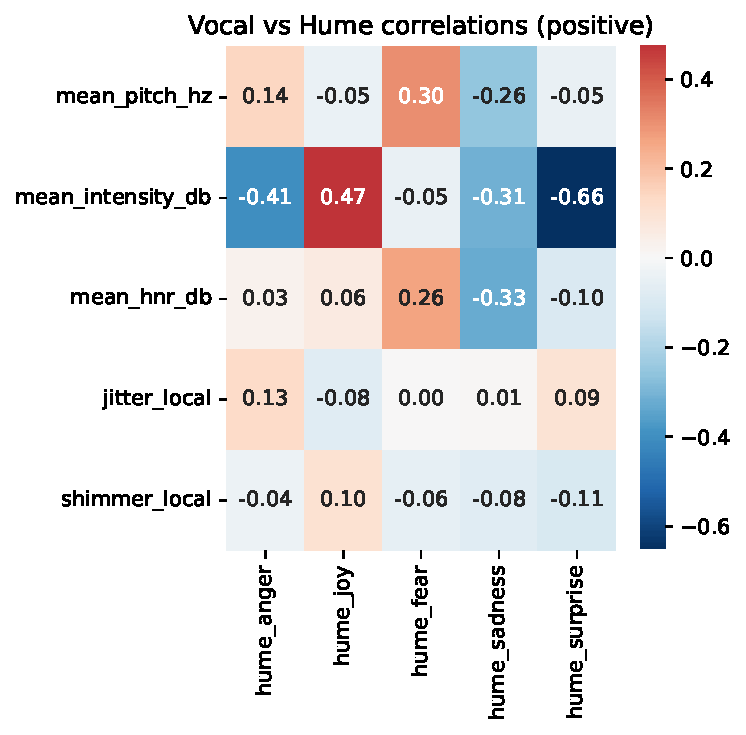
\includegraphics[width=\textwidth]{png/results/rq1_new/vocal_vs_hume_correlations_positive.pdf}
        \caption{Hume vs vocal features positive}
        \label{fig:hume_vocal_positive}
    \end{subfigure}
    \begin{subfigure}[b]{0.45\textwidth}
        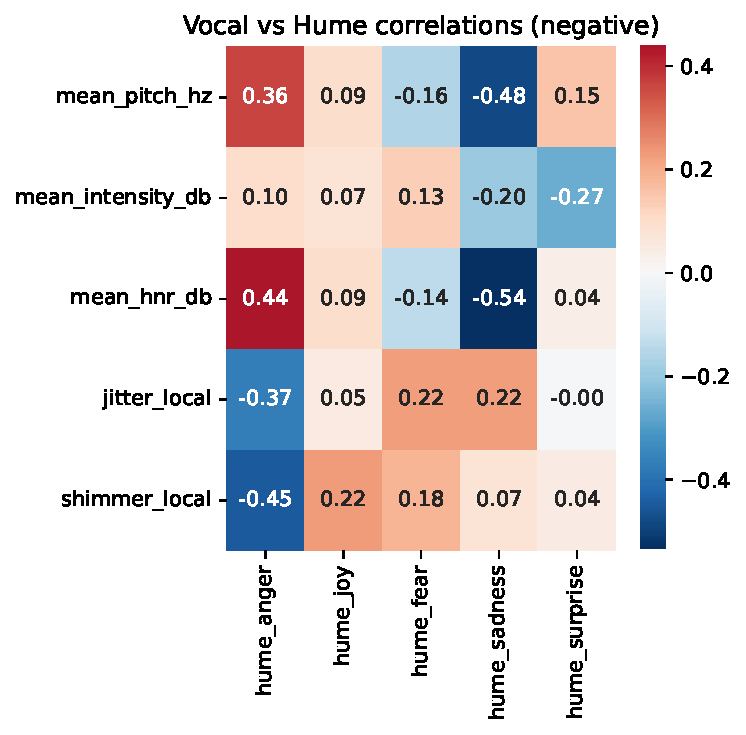
\includegraphics[width=\textwidth]{png/results/rq1_new/vocal_vs_hume_correlations_negative.pdf}
        \caption{Hume vs vocal features negative}        
        \label{fig:hume_vocal_negative}
    \end{subfigure}   
    \caption{Correlation Heatmaps between Hume AI and vocal features.}
    \label{fig:rq1-heatmaps}     
\end{figure}
Correlation values for positive interviews in Figure \ref{fig:hume_vocal_positive} ranging roughly between -0.7 and 0.5, most values suggest generally weaker correlations than the highest values. 
Mean intensity stands out from other vocal features with a moderate positive correlation with Hume Joy (r = 0.47), a moderate negative correlation with Hume Anger (r = -0.41), and a strong negative correlation with Hume Surprise (r = -0.66). 
Mean pitch shows strongest effect on Hume Fear (r = 0.30) and a moderate negative link with Hume Sadness (r = -0.26). 
Mean HNR has a moderate negative correlation with Hume Sadness (r = -0.33) as well it is moderately positively correlated with Hume Fear (r = 0.26). 
Jitter and shimmer remain near zero for most emotions in the positive clips, with none exceeding |r| = 0.13. This suggests that, in more positively oriented interviews, 
variation in pitch, intensity, and HNR capture the core emotion-related cues moderately, while jitter and shimmer have small predictive influence in semi-spontaneous speech during interview conversations. 

Figure \ref{fig:hume_vocal_negative} illustrates Pearson correlation values for negative clips in the dataset, again presenting generally weak effects even if slightly stronger correlations occur, ranging between -0.6 to 0.5. 
The strongest relationship appears for sadness, where mean HNR shows a strong negative correlation (r = -0.54) and pitch has a moderate negative correlation (r = -0.48). The most even distribution of correlation values appear for Hume Anger, 
where all features except intensity shows moderate correlations, most distinct are a positive link with HNR (r = 0.44) and a negative link for shimmer (r = -0.45). Intensity shows overall weak correlations with all emotions, exclusive of Hume Surprise where a moderate negative correlation (r = -0.27) occurs. 
Jitter and shimmer show similar relationships to Hume Fear (r ≈ 0.2). Shimmer has strongest correlation with Hume Anger, and a moderate relationship with Hume Joy. Jitter is moderately correlated with Anger as well and have a moderate correlation with Sadness where shimmer has almost no correlation. 
Pitch and HNR shows the strongest indicators for signalling negative expressed emotions, while intensity measures remain subtle. The slightly strong, but moderate negative correlation between pitch and sadness indicates that the sadder the recording is judged by Hume AI, the lower the average pitch tends to be. 
Both Joy and Surprise has generally weak correlations for all vocal features in the negative oriented clips, which is expected due to these emotions being more positively related. 

\medskip
Overall, the negative and positive diversion suggests that pitch and harmonicity (HNR) consistently reflect Hume AI’s sadness and anger ratings, while intensity mostly marks joy and surprise in positive interviews. Jitter and shimmer remain minor indicators for both interview conditions, except for Anger in the negative clips. 

\subsection{Correlation with Praat-Based Emotion Scores}

\begin{figure}[H]
    \centering 
    \begin{subfigure}[b]{0.45\textwidth}
        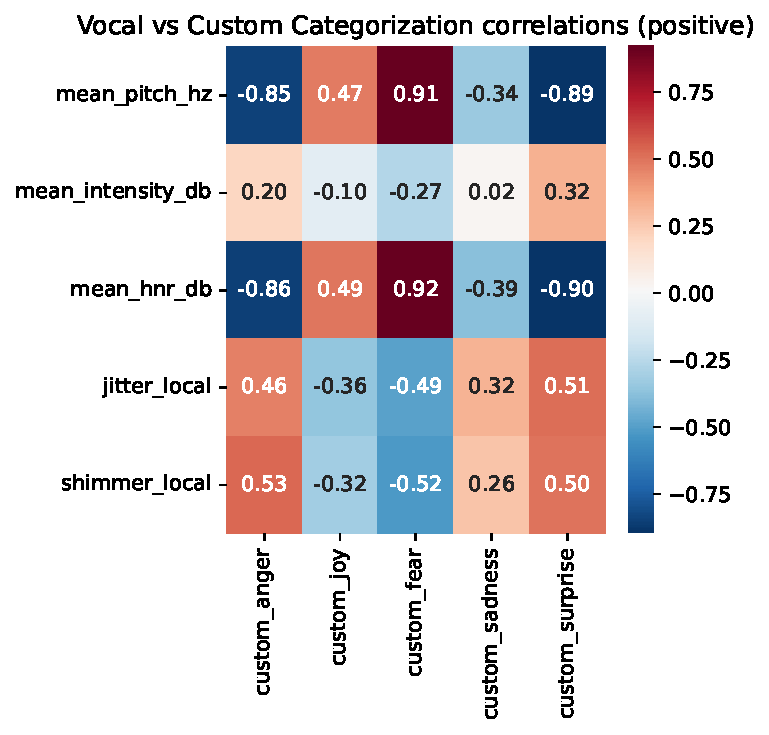
\includegraphics[width=\textwidth]{png/results/rq1_new/vocal_vs_custom_categorization_correlations_positive.pdf}
        \caption{Hume vs custom features positive}
        \label{fig:custom_vocal_positive}
    \end{subfigure}
    \begin{subfigure}[b]{0.45\textwidth}
        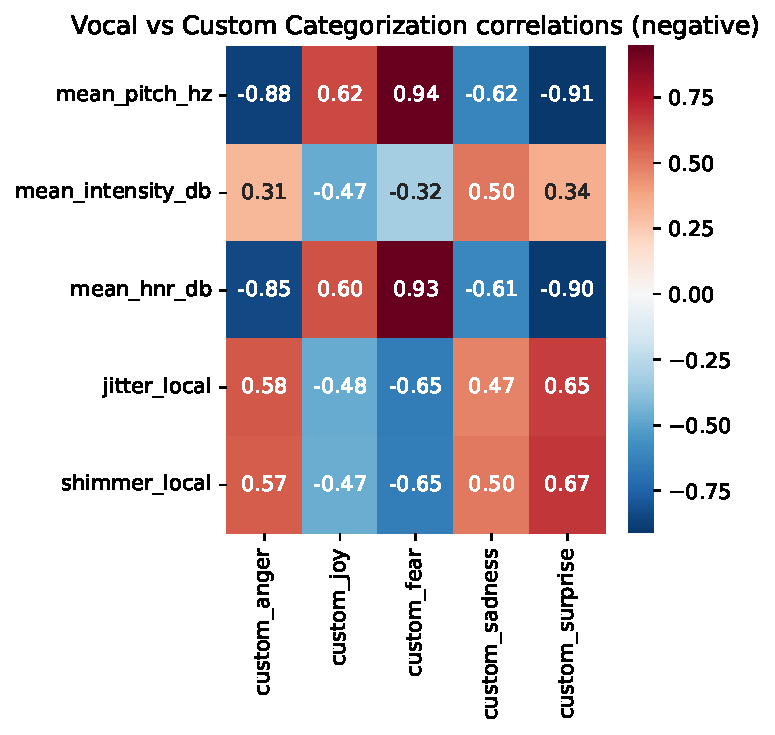
\includegraphics[width=\textwidth]{png/results/rq1_new/vocal_vs_custom_categorization_correlations_negative.pdf}
        \caption{Hume vs custom features negative}        
        \label{fig:custom_vocal_negative}
    \end{subfigure} 
    \caption{Correlation heatmaps between the custom emotion categorization function and vocal features.}
    \label{fig:rq1_heatmaps_custom}       
\end{figure}
Figure~\ref{fig:rq1_heatmaps_custom} presents heatmaps of Pearson’s correlation r between selected vocal features and the emotion scores obtained from the custom emotion categorization 
function for Figure \ref{fig:custom_vocal_positive} positive oriented clips and Figure \ref{fig:custom_vocal_negative} negative clips. Correlations are notably stronger than those observed with the Hume AI labels for both subsets, ranging from -0.9 to 0.95. 
In contrast to the correlation results between Hume AI and vocal markers, these heatmaps presents similar values and orientations for both negative and positive recordings. Pitch and HNR correlations are strongly related for both sentiments, especially between 
pitch and custom categorisations Anger (r = -0.85 and r = -0.88), Fear (r = 0.91 and r = 0.94), and Surprise (r = -0.89 and r = -0.91), the correlation values for HNR is almost identical. Both pitch and HNR shows strong positive correlation for Fear, and strong negative relationship with Anger and Surprise. The almost identical value for these vocal features implies that harmonic clarity is weighted almost identically to pitch in the categorization function, both with a dominant impact on the outcomes of the emotion categorisation. Intensity has a smaller impact, with slightly higher correlations for the negative clips. 
Intensity has weak to moderate relationships across all emotions in the positive recordings, while being strongly correlated with sadness in the negative interviews. The opposite is implied for joy in these interviews, where joy is associated with lower intensity values. 
Jitter and shimmer have slightly stronger correlations across all emotions in the negative oriented clips, yet the values follow the same pattern regarding direction and scale. 

\medskip
These results show that the custom categorization function disproportionately weighted certain vocal features, particularly pitch and HNR, distributing inflating and potentially misleading correlation coefficients. Intensity, shimmer, and jitter has secondary roles with general moderate correlations, although strong correlations appear these features are overwhelmed by pitch and HNR. The almost identical patterns across the sentiment subsets implies overreliance on acoustic features, probably suppressing more subtle cues that are necessary for identifying emotions in semi-spontaneous, conversational speech. 


\subsection{Limitations of the Custom Vocal Emotion Categorization Method}
To evaluate the performance of our custom emotion categorization function, which was developed based on vocal markers reported in the Swedish study \autocite{Ekberg2023}, we compared the emotion labels to the labels generated by Hume AI’s speech-based emotion recognition model. This comparison included both individual clip level and across the full dataset, seperated by sentiment. 

However, the results revealed significant limitations in our approach. Regardless of the vocal input from our dataset, the categorization function consistently rendered near homogeneous emotion scores across all five emotions. This indicates that the function failed to capture emotional distinctions within spontaneous, conversational speech during interviews, regardless of theoretical relevance. 

Figure~\ref{fig:rq1_scatter_hume_praat_pos}, positive, and Figure~\ref{fig:rq1_scatter_hume_praat_neg}, negative, illustrates this issue across the full dataset, where the average scores assigned by our Praat-based categorization remain clustered around 0.2 across all emotions. Opposed to Hume that had greater variation through its labeling and reflects a more dynamic emotional detection.

\begin{figure}[H]
    \centering
    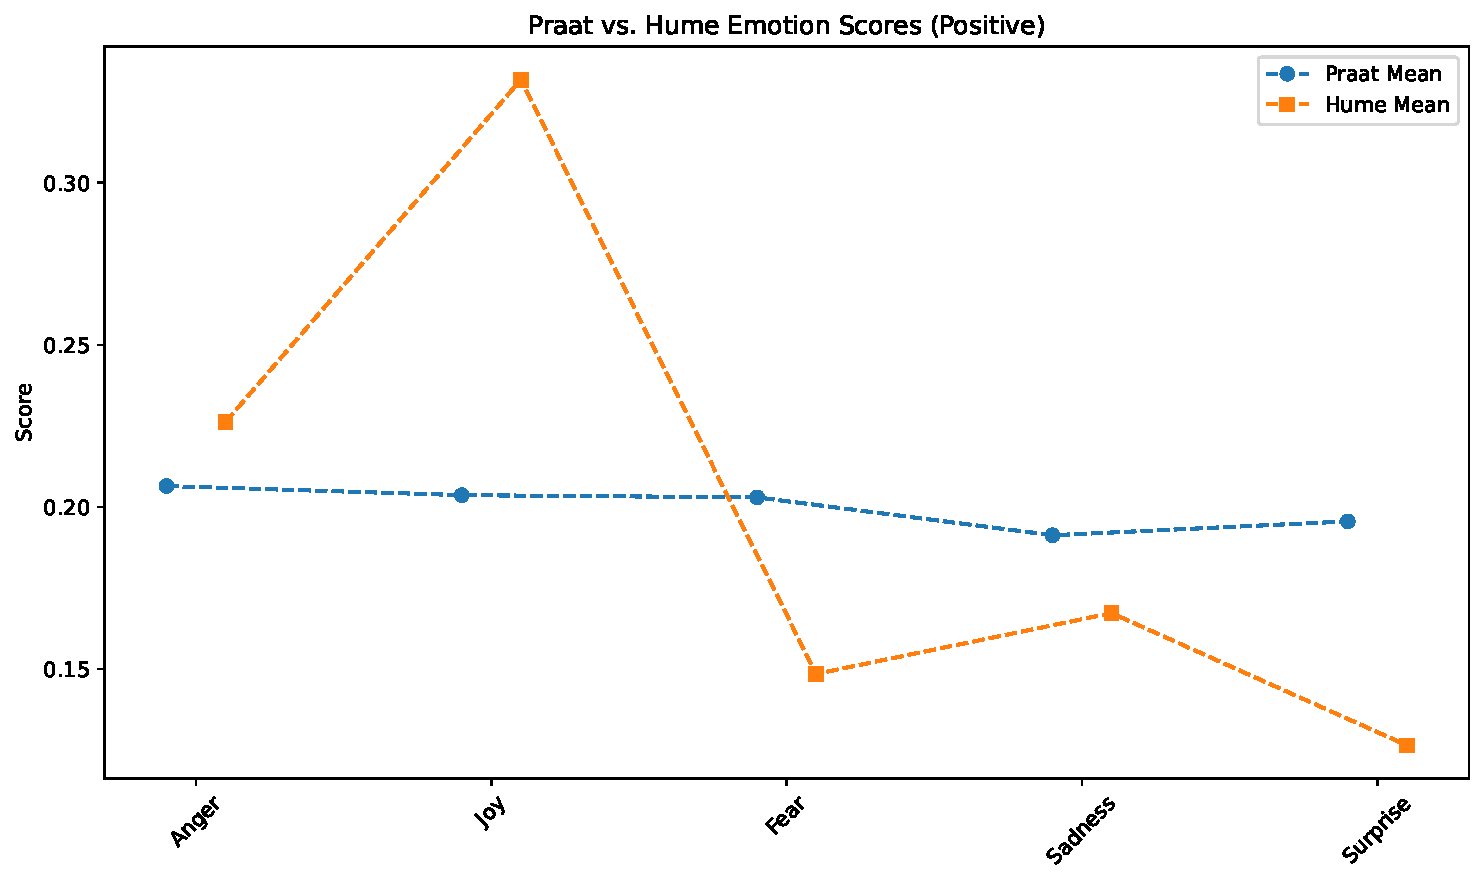
\includegraphics[width=0.75\textwidth]{png/results/rq1_new/praat_hume_positive_scatter.pdf}
    \caption{Average score of custom emotion categorisation function and Hume labeling across positive clips.}
    \label{fig:rq1_scatter_hume_praat_pos}
\end{figure}


\begin{figure}[H]
    \centering
    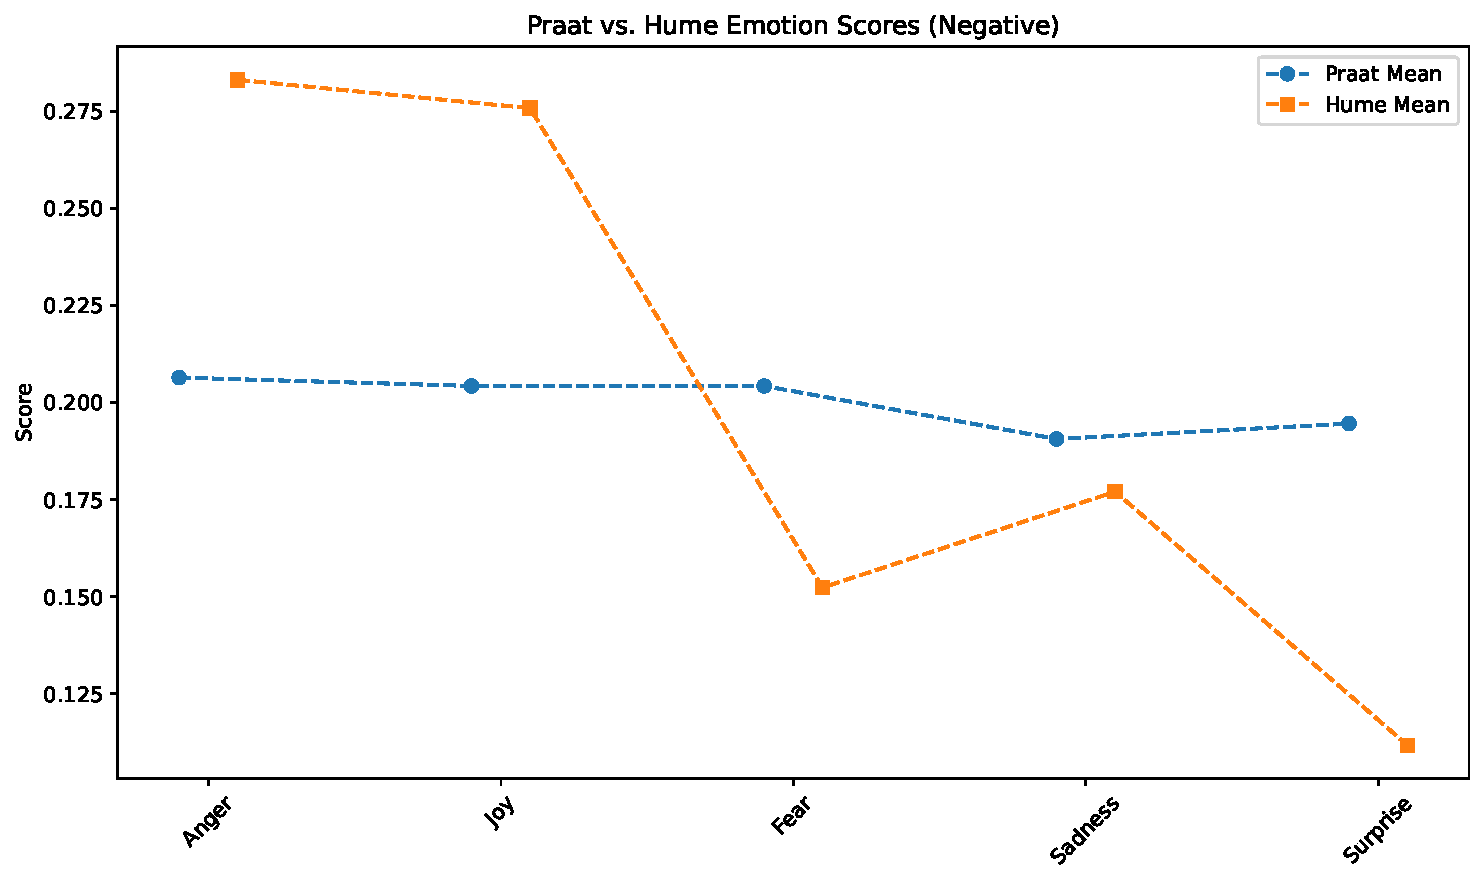
\includegraphics[width=0.75\textwidth]{png/results/rq1_new/praat_hume_negative_scatter.pdf}
    \caption{Average score of custom emotion categorisation function and Hume labeling across negative clips.}
    \label{fig:rq1_scatter_hume_praat_neg}
\end{figure}

    
This is presented similarly in Figure~\ref{fig:praat_hume_006_comb}, which presents a comparison for a single negative 
directed interview \texttt{id\_008\_neg}. In the same way as in Figure~\ref{fig:rq1_scatter_hume_praat_pos} and \ref{fig:rq1_scatter_hume_praat_neg}, 
the Praat-based scores are distributed very evenly across all emotions, while Hume assigns a higher probability to anger and lower for surprise for negative recordings and significantly higher joy scores for positive clips.
Despite the fact that the score diversity between the Hume-labeled emotions are relatively 
moderate, as presented in Figure~\ref{fig:praat_hume_006_comb} comparing one participant's two interviews - approximately 0.05 between anger and fear for the positive clip \ref{fig:praat_hume_006_pos}, yet a differentiation of roughly 0.2 between the highest (fear) and the lowest (surprise) rated emotions. 
The negative interview in Figure~\ref{fig:praat_hume_006_neg} illustrates similar tendencies, with highest probability for anger ($\approx 0.30$) and lowest for surprise (>0.10). 
As both figures in \ref{fig:praat_hume_006_comb} depicts, some alignment occur, yet the probabilities are still more diverse and provide a more interpretable output than yielded from the custom emotion categorisation function. 
The variability could be considered more reflective of potential emotional nuances in the recorded speech. 

These findings demonstrate that our vocal feature-based categorization lacked sensitivity and adaptability when applied to our interview-based Swedish speech data. 
As a result, subsequent analyses focused on direct comparisons between raw vocal features and AI-predicted emotions. 

\begin{figure}[H]
    \centering
    \begin{subfigure}[b]{0.45\textwidth}
        \centering
        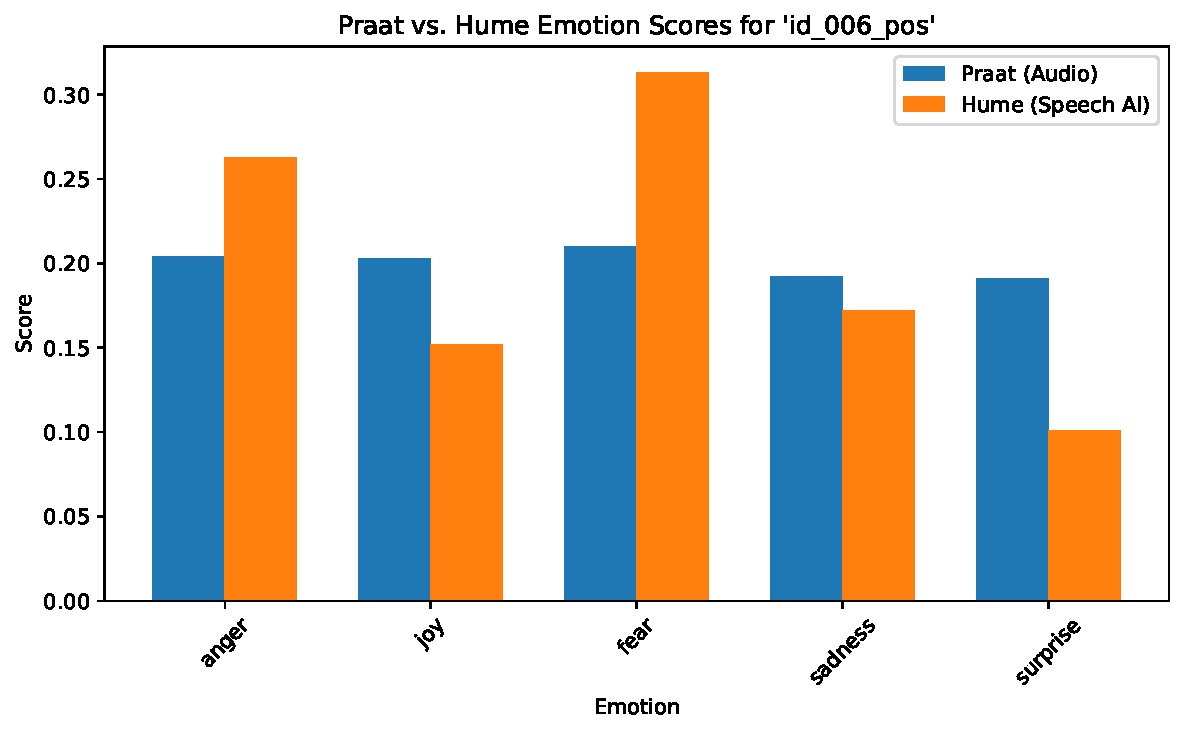
\includegraphics[width=0.7\textwidth]{png/results/rq1_new/id_006_pos_praat_hume_comparison.pdf}
        \caption{Comparison bar single positive clip.}
        \label{fig:praat_hume_006_pos}
    \end{subfigure} 
    \begin{subfigure}[b]{0.45\textwidth}
        \centering
        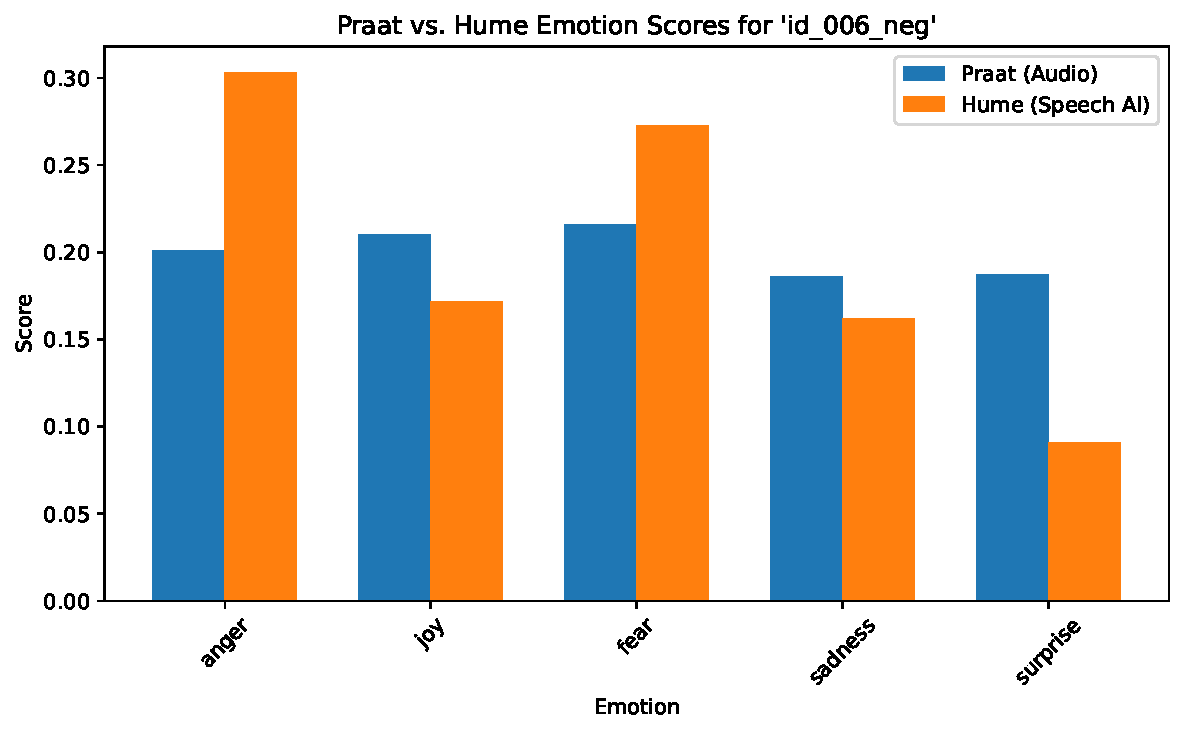
\includegraphics[width=0.7\textwidth]{png/results/rq1_new/id_006_neg_praat_hume_comparison.pdf}
        \caption{Comparison bar single negative clip.}
        \label{fig:praat_hume_006_neg}
    \end{subfigure} 
    \caption{Custom emotion categorization vs. Hume for a single clip (id 006).}
    \label{fig:praat_hume_006_comb}
\end{figure}

\subsection{ANOVA Tables of Vocal Features Across Emotions}
An ANOVA was implemented to further examine whether essential vocal features varied across AI-labeled emotions. This was conducted on pitch, intensity, HNR, jitter, and shimmer. 
The results are summarised in Table~\ref{tab:rq1_anova_pos} for positive recordings and \ref{tab:rq1_anova_neg} for negative recordings, 
showing that none of the features showed statistically significant differences between the five Hume emotion categories (all p-values > 0.30). To confirm these findings, Tukey HSD tests were conducted and resulted in no pairwise comparisons between emotion labels with significant difference. 

\begin{table}[H]
    \centering 
    \begin{subtable}[b]{0.48\textwidth}
        \centering
        \caption*{\textbf{Positive recordings}}
        \begin{tabular}{lrr}
        \toprule
        \multicolumn{1}{c}{\textbf{Feature}} & \textbf{P-value} & \textbf{Significant} \\
        \midrule
        Pitch      & 0,726 & No \\
        Intensity  & 0,812 & No \\
        HNR        & 0,607 & No \\
        Jitter     & 0,954 & No \\
        Shimmer    & 0,731 & No \\
        \bottomrule
        \end{tabular}
        \caption{ANOVA: Positive recordings.}
        \label{tab:rq1_anova_pos}
    \end{subtable}
    \hfill
    \begin{subtable}[b]{0.48\textwidth}
        \centering
        \caption*{\textbf{Negative recordings}}
        \begin{tabular}{lrr}
        \toprule
        \multicolumn{1}{c}{\textbf{Feature}} & \textbf{P-value} & \textbf{Significant} \\
        \midrule
        Pitch      & 0,470 & No \\
        Intensity  & 0,640 & No \\
        HNR        & 0,300 & No \\
        Jitter     & 0,780 & No \\
        Shimmer    & 0,567 & No \\
        \bottomrule
        \end{tabular}
        \caption{ANOVA: Negative recordings.}
        \label{tab:rq1_anova_neg}
    \end{subtable}
    \caption{ANOVA for vocal features across emotions.}
    \label{tab:rq1_anova_all}
\end{table}  
  
These results imply that within our dataset of spontaneous speech during interviews, the average values of the acoustic features did not systematically vary according to AI-labeled emotions. 

OBS! Lägg till medelvärde osv i detta för varje feature (medel och standardavvikelse! )

\subsection{Correlation Between Vocal Features and Hume AI Emotion Scores}
Considering the limitations that had been identified in our vocal feature-based emotion categorization function, subsequent analyses shifted focus towards examining direct correlation between raw acoustic features and AI-predicted emotions. Instead of applying predefined vocal emotion mappings to rely on, essential vocal markers have been investigated to obtain an understanding of how these correlate with Hume AI’s emotion scores across our dataset. 

\subsubsection{Composite Correlation Overview}
Figure~\ref{fig:rq1_composite} illustrates a composite correlation analysis, including Pearson correlation coefficients (r) between two acoustic features, pitch and intensity, and the emotion probabilities from Hume AI. 

\begin{figure}[H]
    \centering 
    \begin{subfigure}[b]{0.48\textwidth}
        \centering
    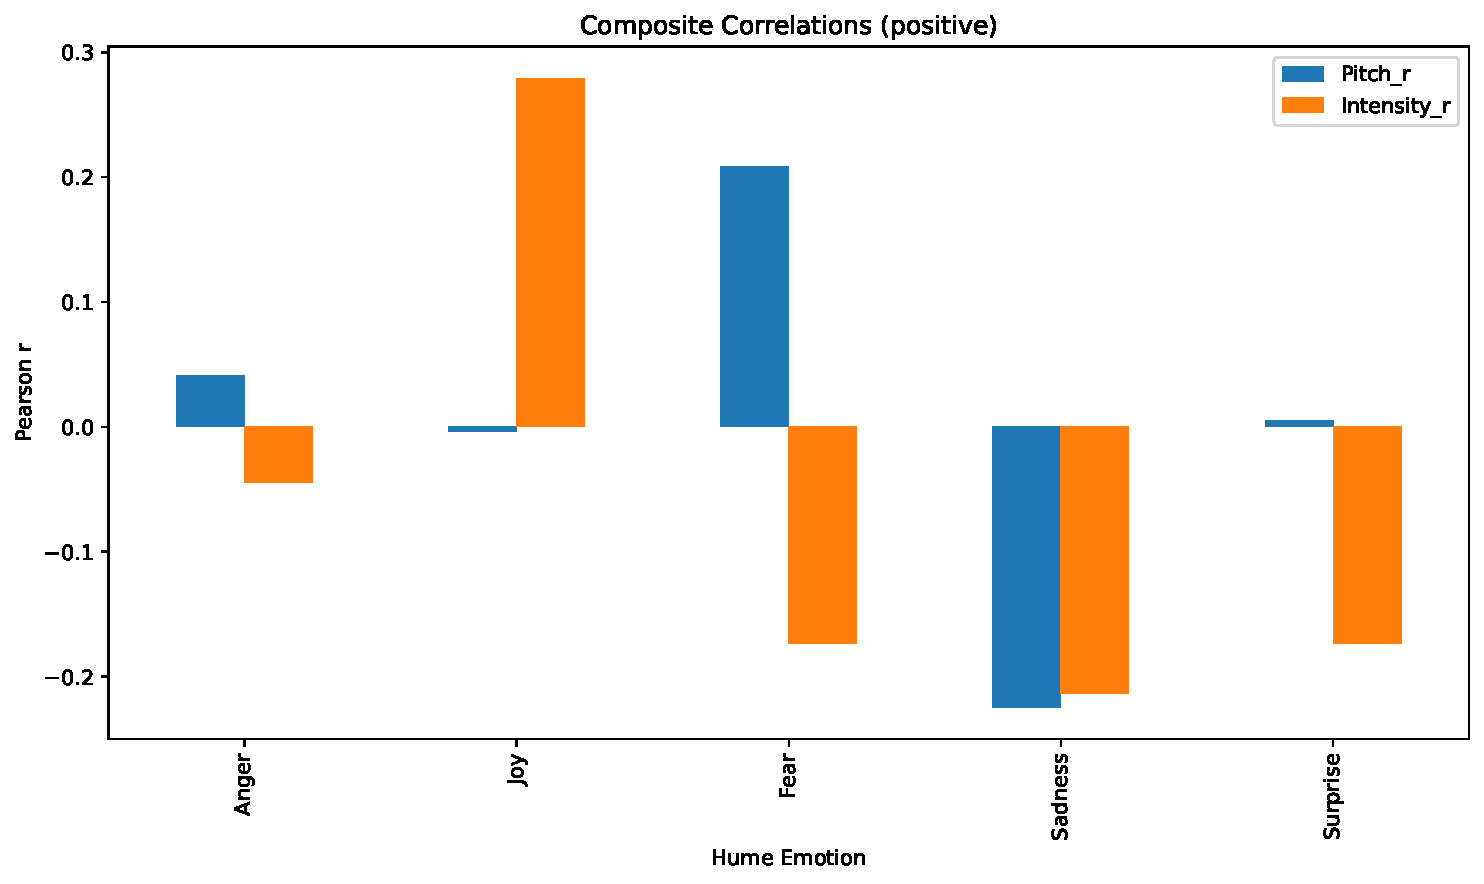
\includegraphics[width=\textwidth]{png/results/rq1_new/composite_correlations_positive.pdf}
    \caption{Positive Recordings}
    \label{fig:rq1_composite_pos}
    \end{subfigure}
    \hfill 
    \begin{subfigure}[b]{0.48\textwidth}
        \centering
        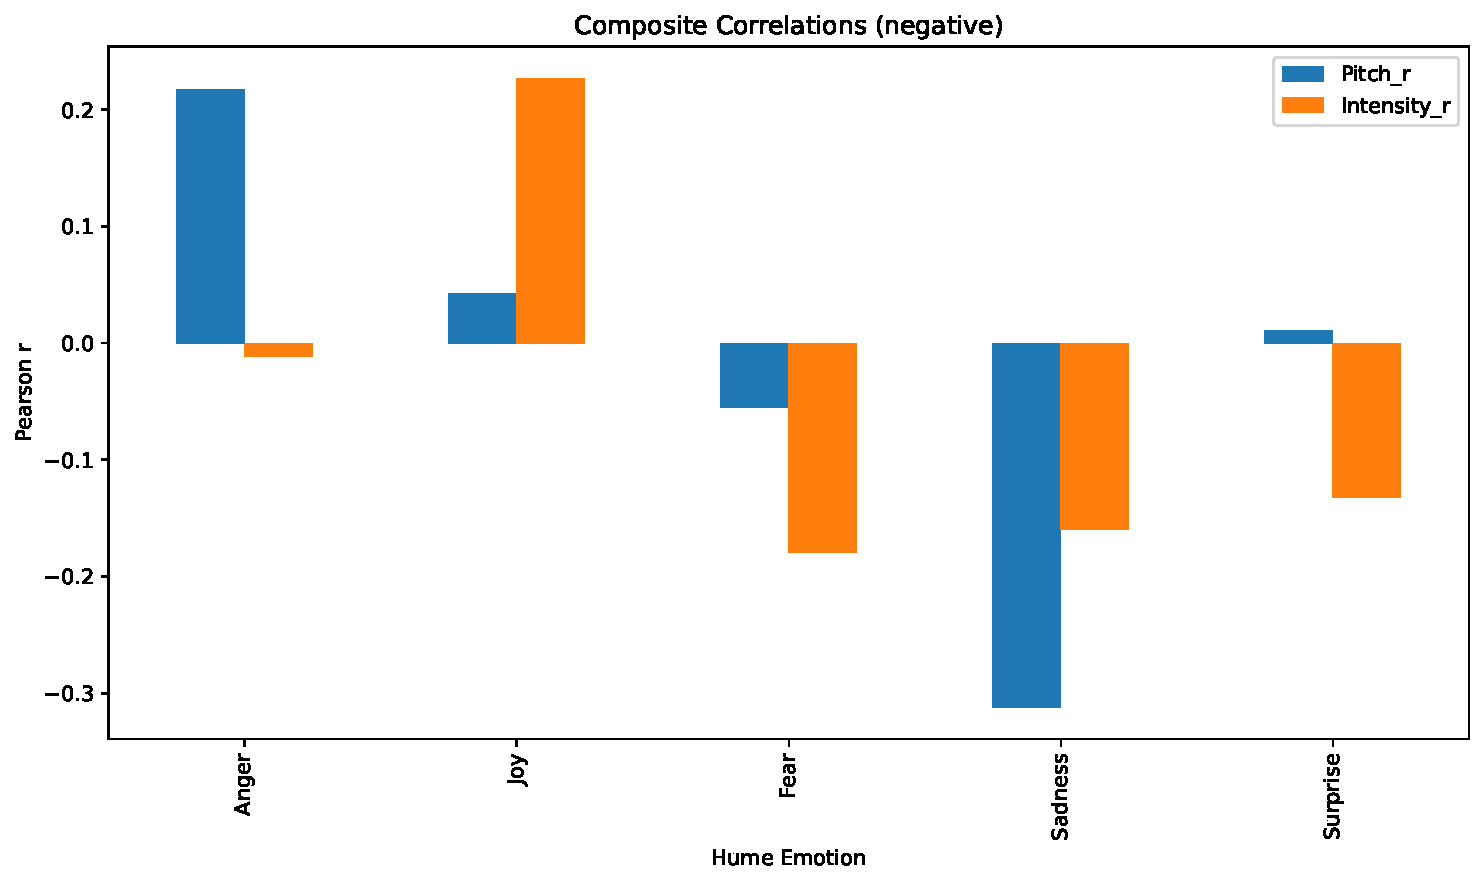
\includegraphics[width=\textwidth]{png/results/rq1_new/composite_correlations_negative.pdf}
    \caption{Negative Recordings}
    \label{fig:rq1_composite_neg}
    \end{subfigure}
    \caption{Composite Correlation diagrams.}
    \label{fig:rq1_composite}
\end{figure}

\begin{table}[H]
    \centering
    \begin{tabular}{lrrrr}
      \toprule
      \textbf{Hume Emotion} & \textbf{Pitch\_r} & \textbf{Pitch\_p} & \textbf{Intensity\_r} & \textbf{Intensity\_p} \\
      \midrule
      Anger    & 0,218 & 0,000 & –0,012 & 0,762 \\
      Joy      & 0,042 & 0,282 &  0,227 & 0,000 \\
      Fear     & –0,055 & 0,159 & –0,180 & 0,000 \\
      Sadness  & –0,312 & 0,000 & –0,160 & 0,000 \\
      Surprise & 0,011 & 0,788 & –0,132 & 0,001 \\
      \bottomrule
    \end{tabular}
    \caption{Correlation coefficients (r) and p-values for pitch and intensity, negative recordings. }
    \label{tab:cor_neg}
  \end{table}
  
Pitch in negative recordings shows a positive correlation with Hume anger (r = 0.218, p < 0.001) and a negative correlation with Hume sadness (r = -0.312, p < 0.001), both showing statistical significance. 
Other emotions presents no significant correlation, where pitch and surprise has the weakest correlation across emotions. Intensity correlates positively with Hume joy (r = 0.227) and had a negative relationship with fear (r = -0.180), sadness (r = -1.60), and surprise (r = -0.132), all statistical significant correlations (p < 0.01). 
Anger was the single emotion showing weak correlation with intensity (r = -0.012, p = 0.762) across the negative interviews. 

  \begin{table}[H]
    \centering
    \begin{tabular}{lrrrr}
      \toprule
      \textbf{Hume Emotion} & \textbf{Pitch\_r} & \textbf{Pitch\_p} & \textbf{Intensity\_r} & \textbf{Intensity\_p} \\
      \midrule
      Anger    & 0,041 & 0,362 & –0,045 & 0,320 \\
      Joy      & –0,004 & 0,936 &  0,279 & 0,000 \\
      Fear     & 0,209 & 0,000 & –0,173 & 0,000 \\
      Sadness  & –0,225 & 0,000 & –0,213 & 0,000 \\
      Surprise & 0,005 & 0,916 & –0,173 & 0,000 \\
      \bottomrule
    \end{tabular}
    \caption{Correlation coefficients (r) and p-values for pitch and intensity, positive recordings. }
    \label{tab:cor_pos}
  \end{table}

Both fear and sadness predicted by Hume AI showed weak correlations with statistical significance with pitch for positive recordings (r = 0.209 and r = -0.225, both p < 0.001). All other pitch correlations were non-significant. 
Intensity correlated most strongly with joy (r = 0.279, p < 0.001), and strongest negatively with sadness (r = -0.213, p < 0.001). Weak correlations with statistical significance were also prevelant between intensity and fear (r = -0.173, p < 0.001) and surprise (r = -0.173, p < 0.001).


\subsubsection{OBS!!! DELETE!!! should be in discussion!!!! }


Particularly intensity shows a positive correlation with joy, and suggests that higher vocal intensity tends to co-occur with AI detected happiness. In contrast, intensity shows a negative correlation with emotions such as sadness and fear, which is aligned with the expectations that these emotions are generally expressed with lower vocal energy. 

For pitch, a minor positive correlation is found in correlation with anger and fear, also reflecting expectations reported in prior research, where higher pitch is associated with heightened arousal states, for example anger. A negative correlation between pitch and sadness is shown, also supporting the prior findings where sadness is linked to lower pitch. 

However, the correlation strength is weak across all emotions, without values that indicate a strong linear association. This indicates, as our previous results, that single acoustic features like pitch and intensity alone are insufficient markers of emotional states when detected by speech emotion recognition systems, in the context of conversational, but interviewed, speech. 

\subsection{Time-to-Time Analysis}

For a more concrete illustration of the prior tendencies , two interview recordings were analyzed in detail. The purpose was to examine whether emotional shifts become more apparent when evaluating shorter time segments within individual speakers, compared to the weaker correlations observed at the dataset level.

\medskip

\begin{figure}[H]
    \centering
    
    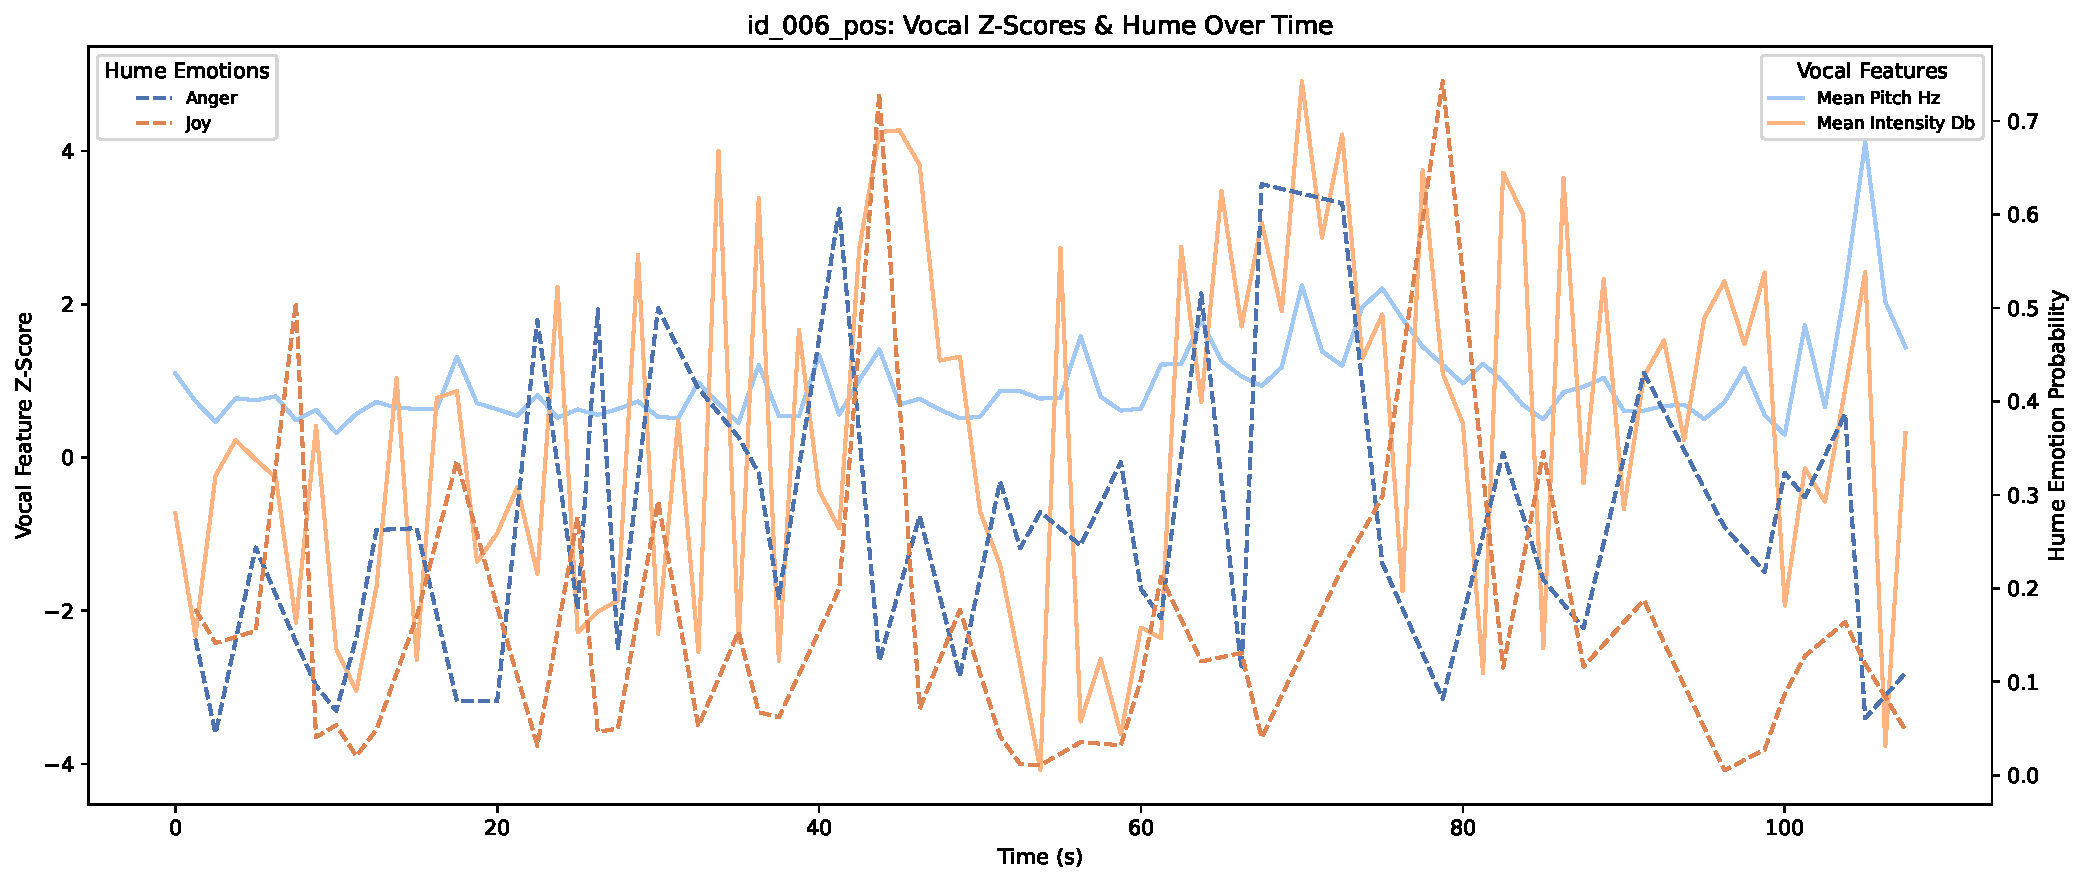
\includegraphics[width=0.85\textwidth]{png/results/rq1_new/006_pos_use_anger-joy.pdf}
    \caption{Pitch and Intensity vs. Hume Anger and Joy. Single positive clip.}
    \label{fig:006_pos-anger-joy}
\end{figure}

\begin{figure}[H]
    \centering
    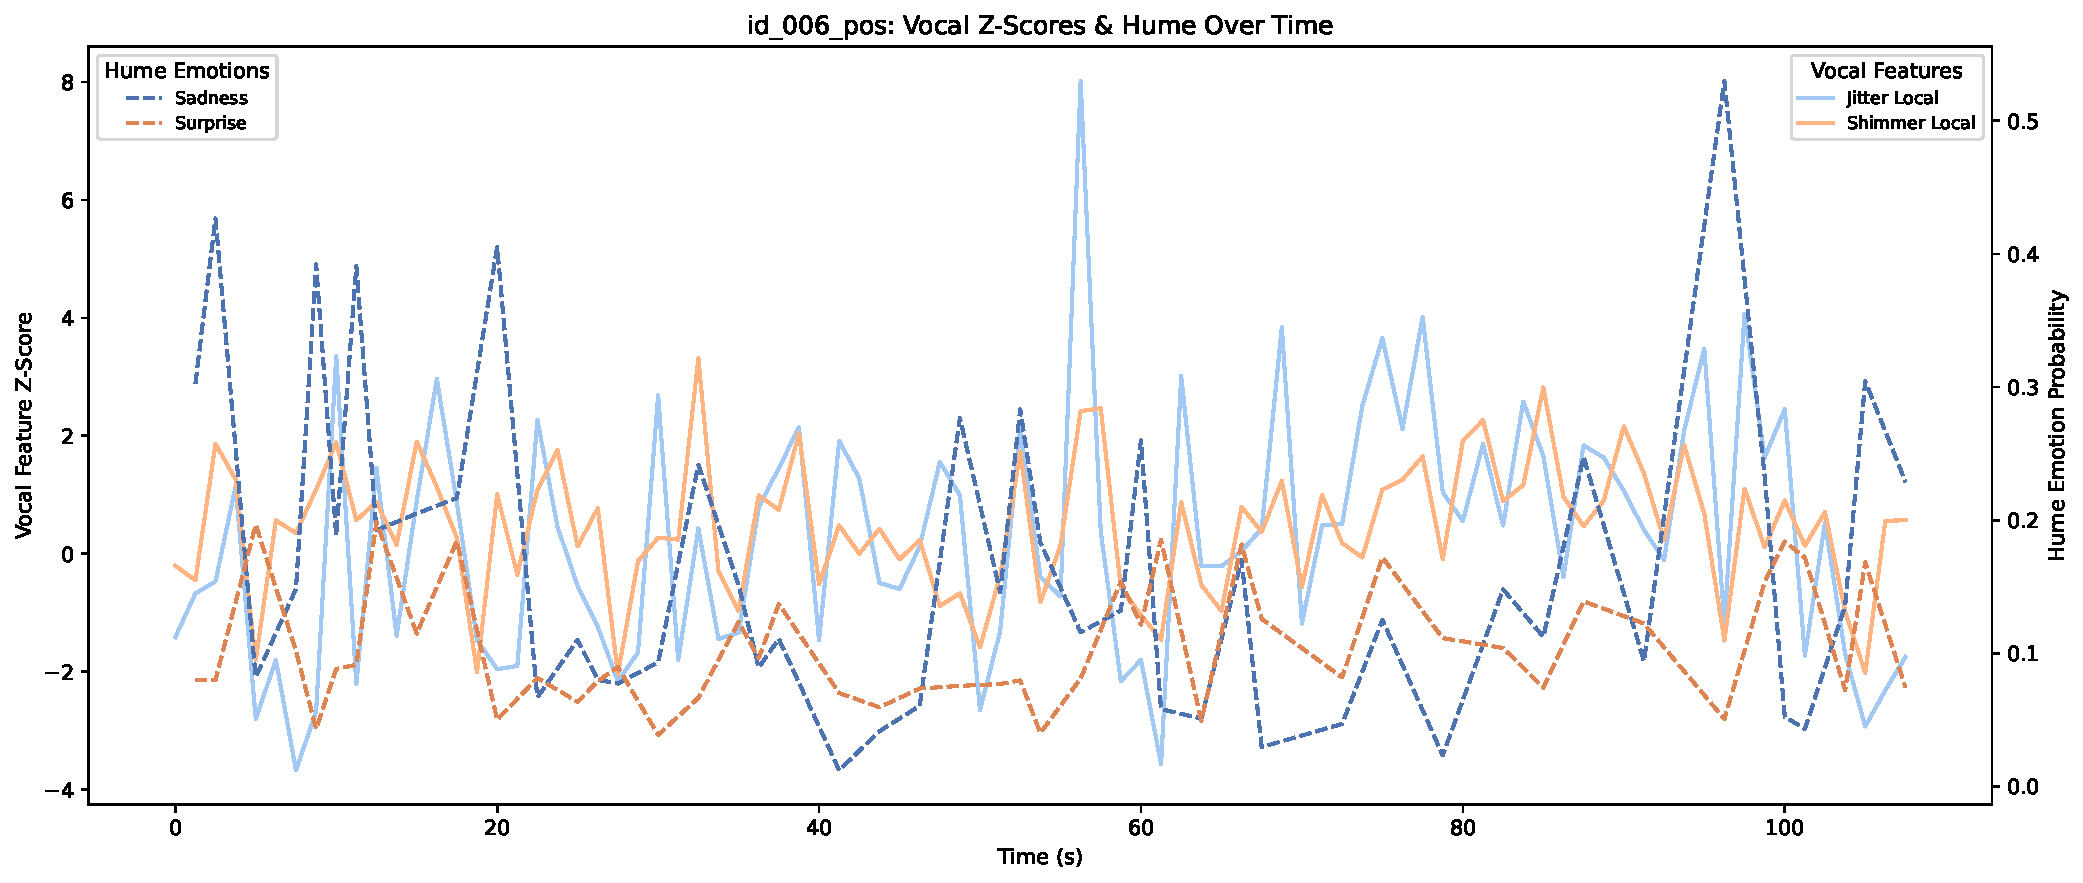
\includegraphics[width=0.85\textwidth]{png/results/rq1_new/006_pos_use-sadn-surp.pdf} 
    \caption{Jitter and Shimmer vs. Hume Sadness and Surprise. Single positive clip.}
    \label{fig:006_pos-surp-sadn}
\end{figure}
    
\begin{table}[H]
    \centering
    %\caption*{\textbf{Significant Correlations}}
    \begin{tabular}{llrr}
        \toprule
        \textbf{Feature}         & \textbf{Emotion} & \textbf{Pearson r} & \textbf{p-value} \\
        \midrule
        mean\_pitch\_st          & surprise         & 0.257              & 0.016            \\
        mean\_pitch\_hz          & surprise         & 0.258              & 0.016            \\
        mean\_intensity\_db      & joy              & 0.271              & 0.011            \\
        mean\_intensity\_db      & fear             & $-0.338$           & 0.001            \\
        \bottomrule
    \end{tabular}
    \caption{Segment-wise Significant Correlations clip 006pos}
    \label{tab:segcorr_significant}
\end{table}

For \ref{tab:segcorr_significant} number of unsignificant: 25 



\begin{table}[H]
    \centering
   % \caption*{\textbf{High vs Low T-tests Statistics}}
    \begin{tabular}{llrr}
        \toprule
        \textbf{Feature}         & \textbf{Emotion} & \textbf{t-statistic} & \textbf{p-value} \\
        \midrule
        mean\_pitch\_st          & surprise         & 2.373                & 0.020            \\
        mean\_pitch\_hz          & surprise         & 2.412                & 0.018            \\
        mean\_intensity\_db      & joy              & 2.399                & 0.019            \\
        \bottomrule
    \end{tabular}
    \caption{High vs Low T-test Statistics (Significant Results) clip 006pos}
    \label{tab:seghighlow_ttest}
\end{table}
  
for \ref{tab:seghighlow_ttest} number unsignificant: 26 


\begin{figure}[H]
    \centering 
    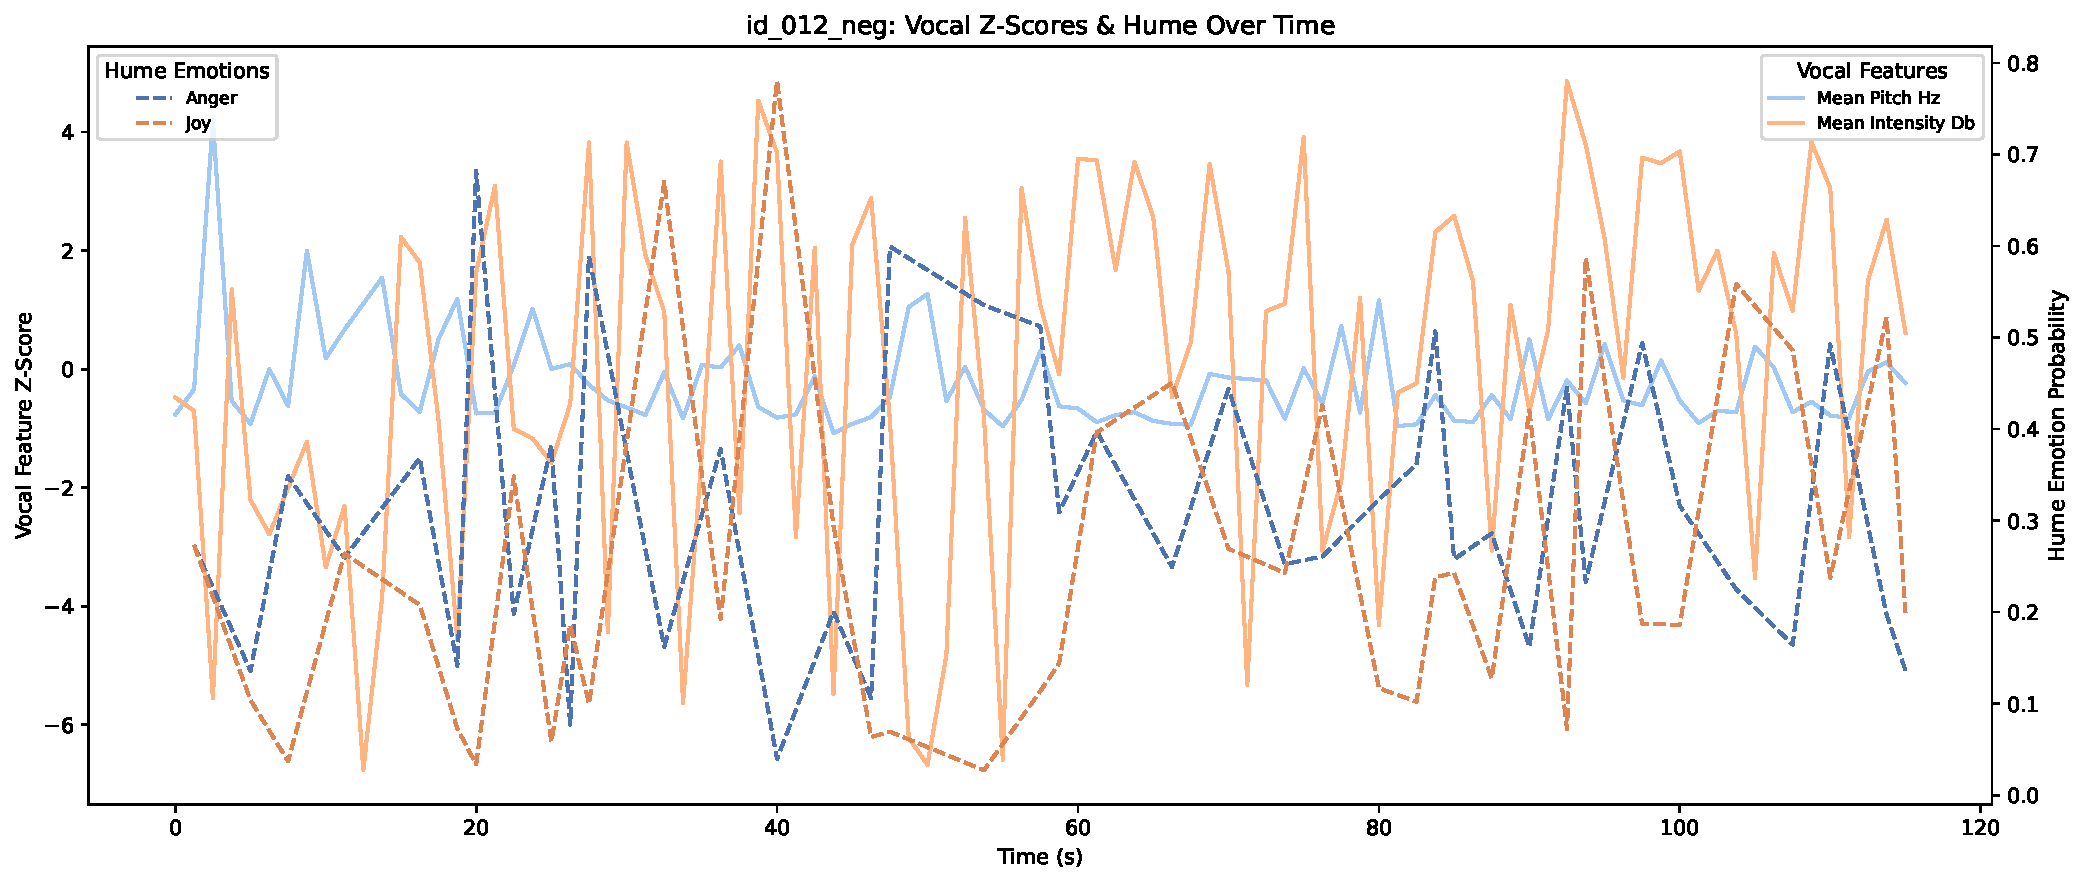
\includegraphics[width=0.85\textwidth]{png/results/rq1_new/012_neg_use-anger-joy.pdf}
    \caption{Z score fluctuation pitch, intensity, anger and joy single clip.}
    \label{fig:z-score-ang-joy-012}
\end{figure}

\begin{figure}[H]
    \centering 
    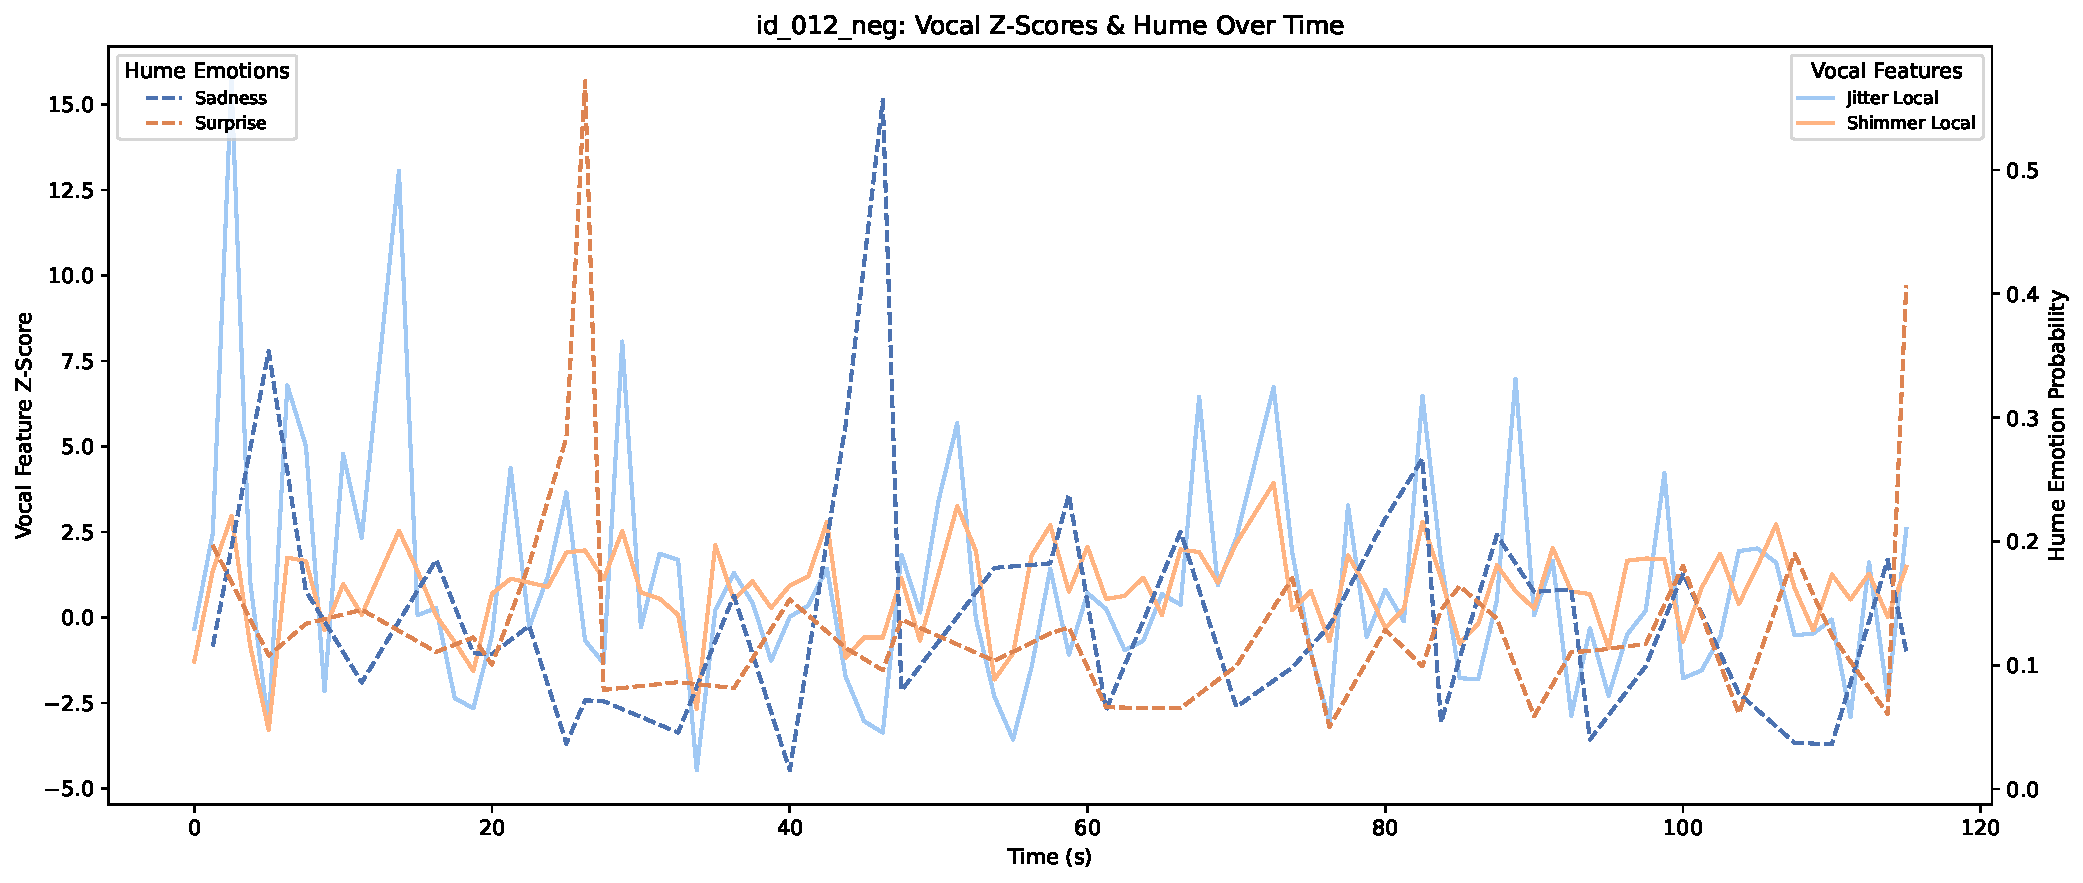
\includegraphics[width=0.85\textwidth]{png/results/rq1_new/012_neg_use-sadn-surp.pdf}
    \caption{Z score fluct jitter, shimmer, sadness, surprise single clip.}
    \label{fig:z-score-surp-sadn-012}
\end{figure}


  \begin{table}[H]
    \centering 
    %\caption*{\textbf{Segment wise correlations : unsig: 25}}
    \begin{tabular}{llrr}
      \toprule
      \textbf{Feature}         & \textbf{Emotion} & \textbf{Pearson r} & \textbf{p-value} \\
      \midrule
      mean\_pitch\_st          & fear             & 0.285              & 0.0063           \\
      mean\_pitch\_hz          & fear             & 0.269              & 0.0099           \\
      mean\_intensity\_db      & fear             & $-0.300$           & 0.0035           \\
      mean\_hnr\_db            & fear             & 0.296              & 0.0040           \\
      mean\_hnr\_db            & surprise         & 0.212              & 0.0417           \\
      \bottomrule
    \end{tabular}
    \caption{Segment-wise Significant Correlations (Fear and Surprise) unsign: 25. clip 012neg}
    \label{tab:segcorr_fear_012}
  \end{table}
  
 
  \begin{table}[H]
    \centering
    \caption*{\textbf{High vs Low T-tests Statistics unsign: 25}}
    \begin{tabular}{llrrr}
      \toprule
      \textbf{Feature}         & \textbf{Emotion} & \textbf{Group}     & \textbf{t-statistic} & \textbf{p-value} \\
      \midrule
      mean\_pitch\_st          & sadness          & High vs Low        & $-2.580$             & 0.0115           \\
      mean\_pitch\_hz          & sadness          & High vs Low        & $-2.343$             & 0.0214           \\
      mean\_hnr\_db            & sadness          & High vs Low        & $-2.397$             & 0.0186           \\
      jitter\_local            & surprise         & High vs Low        & 2.494                & 0.0145           \\
      \bottomrule
    \end{tabular}
    \caption{High vs Low T-test Statistics (Significant Results) unsign: 25 clip 012neg}
    \label{tab:seghighlow_sad_surp_012}
  \end{table}
  



\subsubsection{Time-to-Time Analysis: Full Dataset}
To understand both if acoustic cues correlates with emotion probability by Hume and when they produce clear categorical shifts, two analyses were conducted at time segmened level. 
These effects were observed further with sentiment seperations of all, negative, and positive contexts to see if the emotion-acoustic feature relationship are dependent on positive vs. negative sentiment. 
Table \ref{tab:rq1_time_all_correlations} presents the significant correlations between z-scored acoustic features and Hume emotions.
\begin{table}[H]
    \centering
    \caption*{\textbf{All Recordings}}
    \begin{tabular}{l l r r l}
      \toprule
      \textbf{Feature} & \textbf{Emotion} & \textbf{Pearson’s \(r\)} & \textbf{\(p\)-value} & \textbf{Significant} \\
      \midrule
      mean\_pitch\_hz       & anger      &  0.108  & 0.0003 & Yes \\
      mean\_pitch\_hz       & sadness    & –0.259  & 0.0000 & Yes \\
      mean\_intensity\_db   & joy        &  0.171  & 0.0000 & Yes \\
      mean\_intensity\_db   & fear       & –0.177  & 0.0000 & Yes \\
      mean\_intensity\_db   & sadness    & –0.123  & 0.0000 & Yes \\
      mean\_intensity\_db   & surprise   & –0.119  & 0.0001 & Yes \\
      mean\_hnr\_db         & anger      &  0.126  & 0.0000 & Yes \\
      mean\_hnr\_db         & fear       &  0.076  & 0.0116 & Yes \\
      mean\_hnr\_db         & sadness    & –0.280  & 0.0000 & Yes \\
      jitter\_local         & sadness    &  0.088  & 0.0034 & Yes \\
      \bottomrule
    \end{tabular}
    \caption{Significant Pearson correlations for the full (“all”) dataset.}
    \label{tab:rq1_time_all_correlations}
  \end{table}
 
  Only significant correlation is included. 9 correlations out of 24 indicated significance, the full analysis is presented in Appendix [FIGURE REF]. 
  All correlations are perceived as weak even if there is statistical significance. Pitch correlated positively with anger (r = 0.108), and negatively with sadness (r = -0.259). 
  Intensity had a increased relationship with joy (r = 0.171), but decreased with fear (r = -0.177), sadness (r = -0.123) and surprise (r = -0.119). HNR showed a weak positive correlation with anger (r = 0.126) and fear (r = 0.076), and a negative correlation with sadness (r = -0.280). 
  Jitter had a single significant, yet weak correlation with sadness (r = 0.088). Shimmer showed no significant correlations. 

Table \ref{tab:ttest_full_features} compares the top 30\% and bottom 70\% of emotion-probability time-segments, and tests wheather the mean z-scored feature differs between the high vs. low groups. 
A large t-statistic value indicate a reliable shift in that feature when Hume rates that emotion high. 
\begin{table}[H]
    \centering
    \caption{High-vs-low t-test results for significant acoustic features (full dataset)}
    \begin{tabular}{l l r r l}
      \toprule
      \textbf{Feature} & \textbf{Emotion} & \textbf{t-statistic} & \textbf{\(p\)-value} & \textbf{Significant?} \\
      \midrule
      mean\_pitch\_hz       & anger     &  4.533 & 0.0000 & Yes \\
      mean\_pitch\_hz       & sadness   & –8.973 & 0.0000 & Yes \\
      mean\_intensity\_db   & joy       &  5.018 & 0.0000 & Yes \\
      mean\_intensity\_db   & fear      & –4.035 & 0.0001 & Yes \\
      mean\_intensity\_db   & sadness   & –3.285 & 0.0011 & Yes \\
      mean\_intensity\_db   & surprise  & –3.646 & 0.0003 & Yes \\
      mean\_hnr\_db         & anger     &  4.547 & 0.0000 & Yes \\
      mean\_hnr\_db         & fear      &  3.839 & 0.0001 & Yes \\
      mean\_hnr\_db         & sadness   & –8.698 & 0.0000 & Yes \\
      jitter\_local         & sadness   &  1.808 & 0.0709 & No  \\
      \bottomrule
    \end{tabular}
    \label{tab:ttest_full_features}
  \end{table}
  
  High-anger predictions of segmented recordings had significanty higher pitch (t = 4.52) and HNR (t = 4.55). 
  High-sadness segments show increased pitch (t = -8.97), intensity (t = -3.29), HNR (t = -8.70), and a small, not significant increase in jitter (t = 1.81, p = 0.0709).
  Joy segments have higher intensity (t = 5.02), while fear segments have lower intensity (t = -4.04) and increased HNR (t = 3.84). 
  Segments with high surprise predictions has the moderately low intensity (t = -3.646). 
  
  \subsubsection{Time-to-Time Analysis by Sentiment}
  \begin{table}[H]
    \centering
    \begin{subtable}{0.45\textwidth}
      \centering
      \caption{Pitch and Anger (Pearson \(r\))}\label{tab:rq1_corr_pitch_anger}
      \begin{tabular}{l r r l}
        \toprule
        Sentiment & \(\;r\;\) & \(\;p\;\) & Sig? \\
        \midrule
        all      &  0.108 & 0.0003 & Yes \\
        negative &  0.194 & 0.0000 & Yes \\
        positive & -0.024 & 0.6049 & No  \\
        \bottomrule
      \end{tabular}
    \end{subtable}\hfill
    \begin{subtable}{0.45\textwidth}
      \centering
      \caption{Pitch and Anger (t-test)}\label{tab:rq1_ttest_pitch_anger}
      \begin{tabular}{l r r l}
        \toprule
        Sentiment & \(\;t\;\) & \(\;p\;\) & Sig? \\
        \midrule
        all      &  4.533 & 0.0000 & Yes \\
        negative &  4.836 & 0.0000 & Yes \\
        positive &  1.353 & 0.1767 & No  \\
        \bottomrule
      \end{tabular}
    \end{subtable}
    \caption{(a) Pearson correlations and (b) high-vs-low t-test results for pitch vs. anger by sentiment.}
    \label{tab:rq1_pitch_anger_side_by_side}
  \end{table}
  
  Table \ref{tab:rq1_pitch_anger_side_by_side} presents that pitch shows a weak but significant positive correlation with anger for the full dataset (r = 0.108, p < 0.001), and in negative recordings (p = 0.194, p < 0.001), but not in positive clips (p = -0.024, p = 0.605). 
  The t-tests in \ref{tab:rq1_ttest_pitch_anger} confirms this where high-anger segments have markedly higher pitch in the full dataset (t = 4.53, p < 0.001) and in negative (t = 4.84, p < 0.001), but not in positive clips (t = 1.35, p = 0.177).
  This implies that pitch really signals anger when the overall context is negative. 

  \begin{table}[H]
    \centering
  
    %%% HNR ⇔ Anger block %%%
    \begin{subtable}{0.45\textwidth}
      \centering
      \caption{HNR and Anger (r)}\label{tab:rq1_corr_hnr_anger}
      \begin{tabular}{l r r l}
        \toprule
        Sentiment & \(\;r\;\) & \(\;p\;\) & Sig? \\
        \midrule
        all      & 0.126 & 0.0000 & Yes \\
        negative & 0.193 & 0.0000 & Yes \\
        positive & 0.009 & 0.8514 & No  \\
        \bottomrule
      \end{tabular}
    \end{subtable}\hfill
    \begin{subtable}{0.45\textwidth}
      \centering
      \caption{HNR and Anger (t-test)}\label{tab:rq1_ttest_hnr_anger}
      \begin{tabular}{l r r l}
        \toprule
        Sentiment & \(\;t\;\) & \(\;p\;\) & Sig? \\
        \midrule
        all      & 4.547 & 0.0000 & Yes \\
        negative & 4.800 & 0.0000 & Yes \\
        positive & 1.891 & 0.0593 & No  \\
        \bottomrule
      \end{tabular}
    \end{subtable}
  
    \caption{HNR–Anger correlations and t-test results by sentiment.}
    \label{tab:rq1_hnr_anger_side_by_side}
  \end{table}
  
  Table \ref{tab:rq1_hnr_anger_side_by_side} presents harmonic-to-noise correlation with anger for the full dataset (r = 0.126, p < 0.001), implying a significant but weak relationship. 
  T-tests in \ref{tab:rq1_ttest_hnr_anger} shows that HNR distinguish high vs low anger for both the full and negative dataset (t = 4.55, t = 4.80 respectively).
  The correlation is significant, still weak, in negative contexts (r = 0.193, p < 0.001) but non-significant in positive recordings (r = 0.009, p = 0.851), which also has a non-significant distinction in the t-tests.
  Together with pitch, HNR appears to be the most prevalent features correlated with anger in negative circumstances. 
  
  \begin{table}[H]
    \centering
  
    %%% Pitch ⇔ Joy block %%%
    \begin{subtable}{0.45\textwidth}
      \centering
      \caption{Pitch and Joy (r)}\label{tab:rq1_corr_pitch_joy}
      \begin{tabular}{l r r l}
        \toprule
        Sentiment & \(\;r\;\) & \(\;p\;\) & Sig? \\
        \midrule
        all      & 0.048 & 0.1067 & No  \\
        negative & 0.005 & 0.8912 & No  \\
        positive & 0.103 & 0.0226 & Yes \\
        \bottomrule
      \end{tabular}
    \end{subtable}\hfill
    \begin{subtable}{0.45\textwidth}
      \centering
      \caption{Pitch and Joy (t-test)}\label{tab:rq1_ttest_pitch_joy}
      \begin{tabular}{l r r l}
        \toprule
        Sentiment & \(\;t\;\) & \(\;p\;\) & Sig? \\
        \midrule
        all      & 2.320 & 0.0205 & Yes \\
        negative & 0.847 & 0.3972 & No  \\
        positive & 1.771 & 0.0772 & No  \\
        \bottomrule
      \end{tabular}
    \end{subtable}
  
    \caption{Pitch–Joy correlations and t-test results by sentiment.}
    \label{tab:rq1_pitch_joy_side_by_side}
  \end{table}
  
  Pitch and joy correlations is presented in Table~\ref{tab:rq1_pitch_joy_side_by_side}, showing unlike anger, a weak correlation for the full dataset (r = 0.048, p = 0.1067). 
  Pitch reaches a weak, but significant correlation with joy in positive recordings (r = 0.103, p = 0.023) and no significance in the negative subset. 
  The t-tests is only significant in the full dataset (t = 2.320, p = 0.021), not for the positive clips (t = 1.771, p = 0.077), implying a more context-specific and non-linear affect.
  
  \begin{table}[H]
    \centering
  
    %%% Intensity ⇔ Joy block %%%
    \begin{subtable}{0.45\textwidth}
      \centering
      \caption{Intensity and Joy (r)}\label{tab:rq1_corr_intensity_joy}
      \begin{tabular}{l r r l}
        \toprule
        Sentiment & \(\;r\;\) & \(\;p\;\) & Sig? \\
        \midrule
        all      & 0.171 & 0.0000 & Yes \\
        negative & 0.149 & 0.0002 & Yes \\
        positive & 0.192 & 0.0000 & Yes \\
        \bottomrule
      \end{tabular}
    \end{subtable}\hfill
    \begin{subtable}{0.45\textwidth}
      \centering
      \caption{Intensity and Joy (t-test)}\label{tab:rq1_ttest_intensity_joy}
      \begin{tabular}{l r r l}
        \toprule
        Sentiment & \(\;t\;\) & \(\;p\;\) & Sig? \\
        \midrule
        all      & 5.018 & 0.0000 & Yes \\
        negative & 2.701 & 0.0071 & Yes \\
        positive & 3.757 & 0.0002 & Yes \\
        \bottomrule
      \end{tabular}
    \end{subtable}
  
    \caption{Intensity–Joy correlations and t-test results by sentiment.}
    \label{tab:rq1_intensity_joy_side_by_side}
  \end{table}
Table \ref{tab:rq1_intensity_joy_side_by_side} demonstrates the correlation between intensity and joy, showing stronger associations compared to joy and pitch. 
All contexts show a positive relationship, strongest for positive clips (r = 0.192, p < 0.001) with significant mean differences where the full dataset has highest significance (t = 5.02, p < 0.001). 
These results suggests that intensity is a stable cue to joy regardless of the overall sentiment context, even if higher correlation occurs for the full and positive sets than the negative subset (r = 0.149, p < 0.001 and t = 2.701, p = 0.007). 

\subsubsection{Pitch and Hume emotion over time}
In Figure~\ref{fig:pitch-4-pos} and \ref{fig:intensity-4-pos}, data is demonstrated from a positively directed interview \texttt{id\_004\_pos}, female, which shows that increases in pitch and intensity considerably often correlate with higher joy probabilities by Hume AI. While the correlation is not consistent throughout the recording, these moment-to-moment variations reflect the general expectation that higher vocal energy is associated with positive emotional expression. 

\begin{figure}[H]
    \centering
    \begin{subfigure}[b]{0.47\textwidth}
        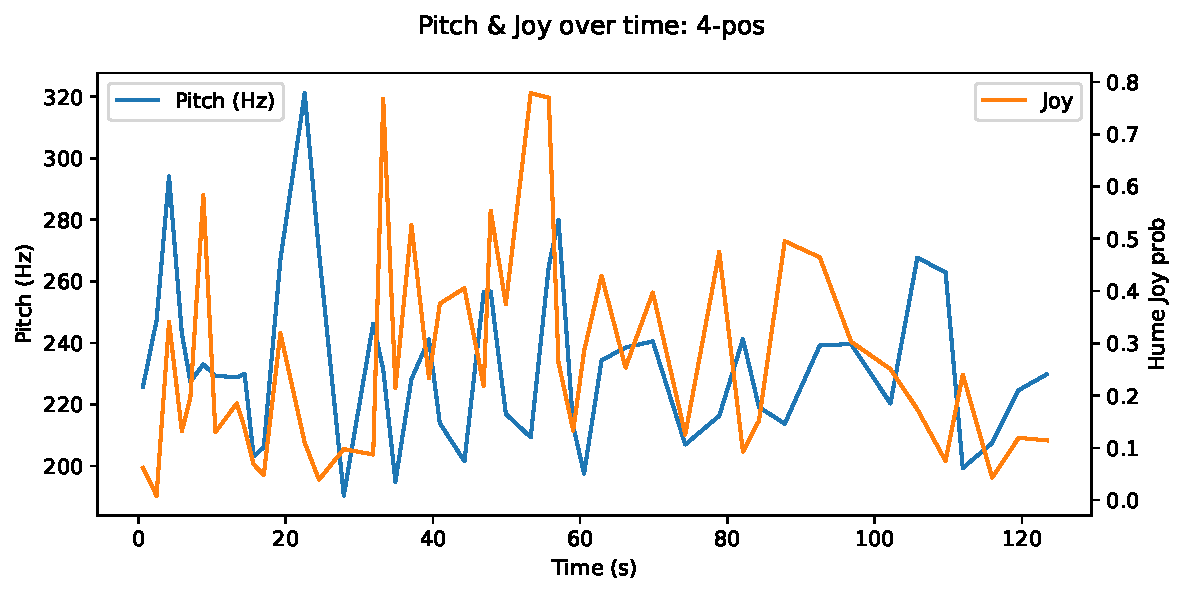
\includegraphics[width=\linewidth]{png/results/rq1/pitch_joy_4-pos.pdf}
        \caption{Pitch(Hz) and Hume label joy over time. Clip 4-pos}
        \label{fig:pitch-4-pos}
    \end{subfigure}
    \hspace{0.04\textwidth}
    \begin{subfigure}[b]{0.47\textwidth}
        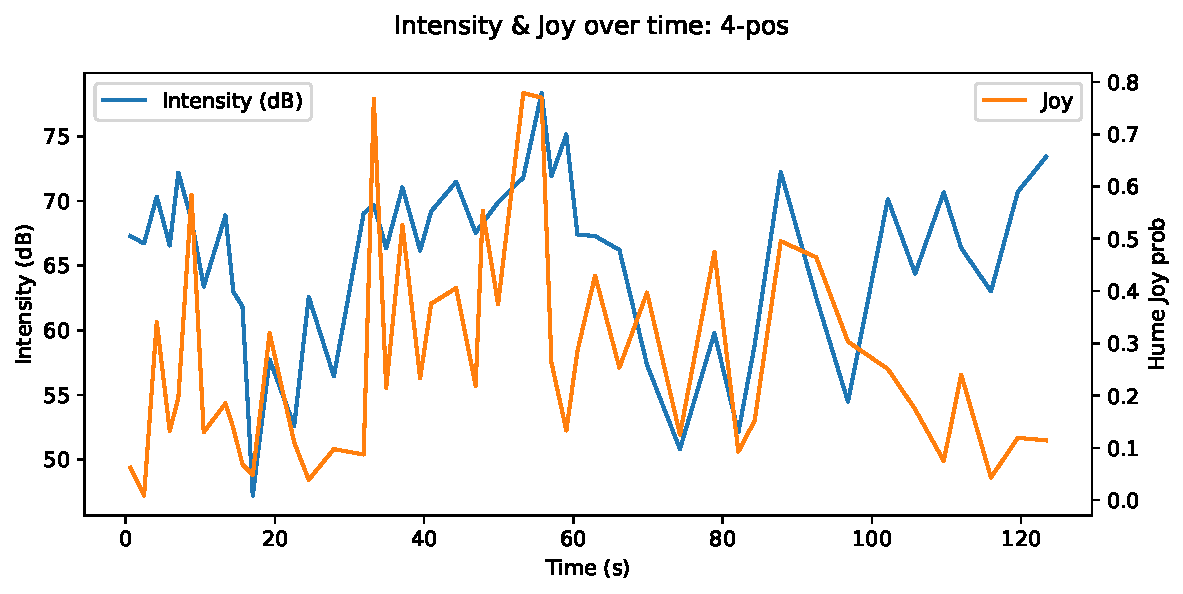
\includegraphics[width=\linewidth]{png/results/rq1/intensity_joy_4-pos.pdf}
        \caption{Intensity(dB) and Hume label joy over time. Clip 4-pos}
        \label{fig:intensity-4-pos}
    \end{subfigure}
\end{figure}

Similarly, Figure~\ref{fig:pitch-15-neg} and \ref{fig:intensity-15-neg} and \ref{fig:z-score-15} present data from a negatively directed interview \texttt{id\_015\_neg}, male. Here, clear peaks in pitch and intensity correspond with increased anger probabilities. These results are partly aligned with prior research on vocal markers of high-arousal negative emotions, such as raised pitch and loudness during expressed anger. 

\begin{figure}[H]
    \centering
    \begin{subfigure}[b]{0.47\textwidth}
        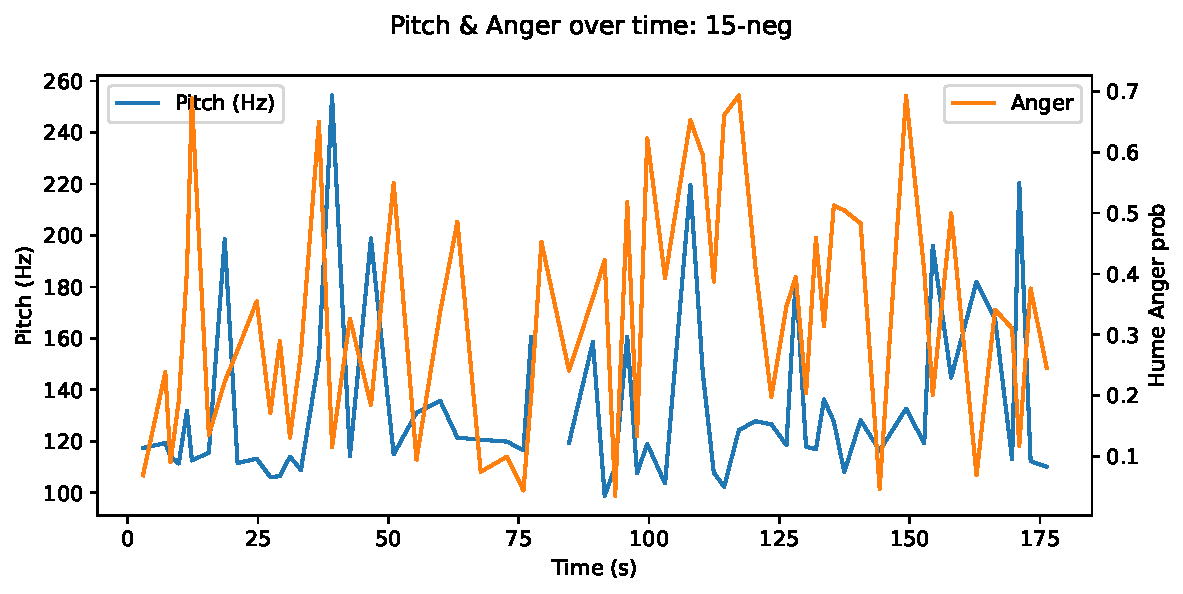
\includegraphics[width=\linewidth]{png/results/rq1/pitch_anger_15-neg.pdf}
        \caption{Pitch(Hz) and Hume label joy over time. Clip 15-neg}
        \label{fig:pitch-15-neg}
    \end{subfigure}
    \hspace{0.04\textwidth}
    \begin{subfigure}[b]{0.47\textwidth}
        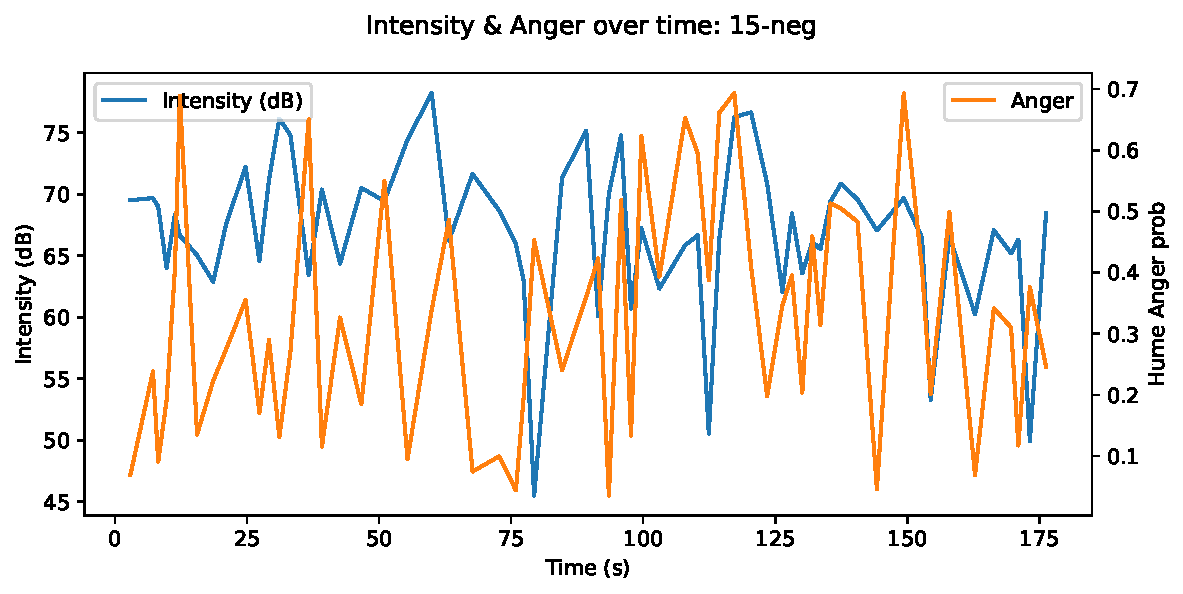
\includegraphics[width=\linewidth]{png/results/rq1/intensity_anger_15-neg.pdf}
        \caption{Intensity(dB) and Hume label joy over time. Clip 15-neg}
        \label{fig:intensity-15-neg}
    \end{subfigure}
\end{figure}

Additionally, Figure \ref{fig:z-score-15} illustrates z-score fluctuations of key vocal features for clip 13-neg. For this interview, several segments exceed +-1 standard deviation from the baseline, especially for pitch, intensity, and shimmer. These flagged moments align frequently with the emotion probabilities of Hume, which strengthens the link between vocal patterns and perceived emotional intensity. 

The z-score fluctuation diagram Figure \ref{fig:z-score-15} illustrates the segments further where vocal features significantly deviate from baseline levels, in patterns aligned with associated high-arousal negative emotions such as raised pitch and loudness. 

\begin{figure}[H]
    \centering 
    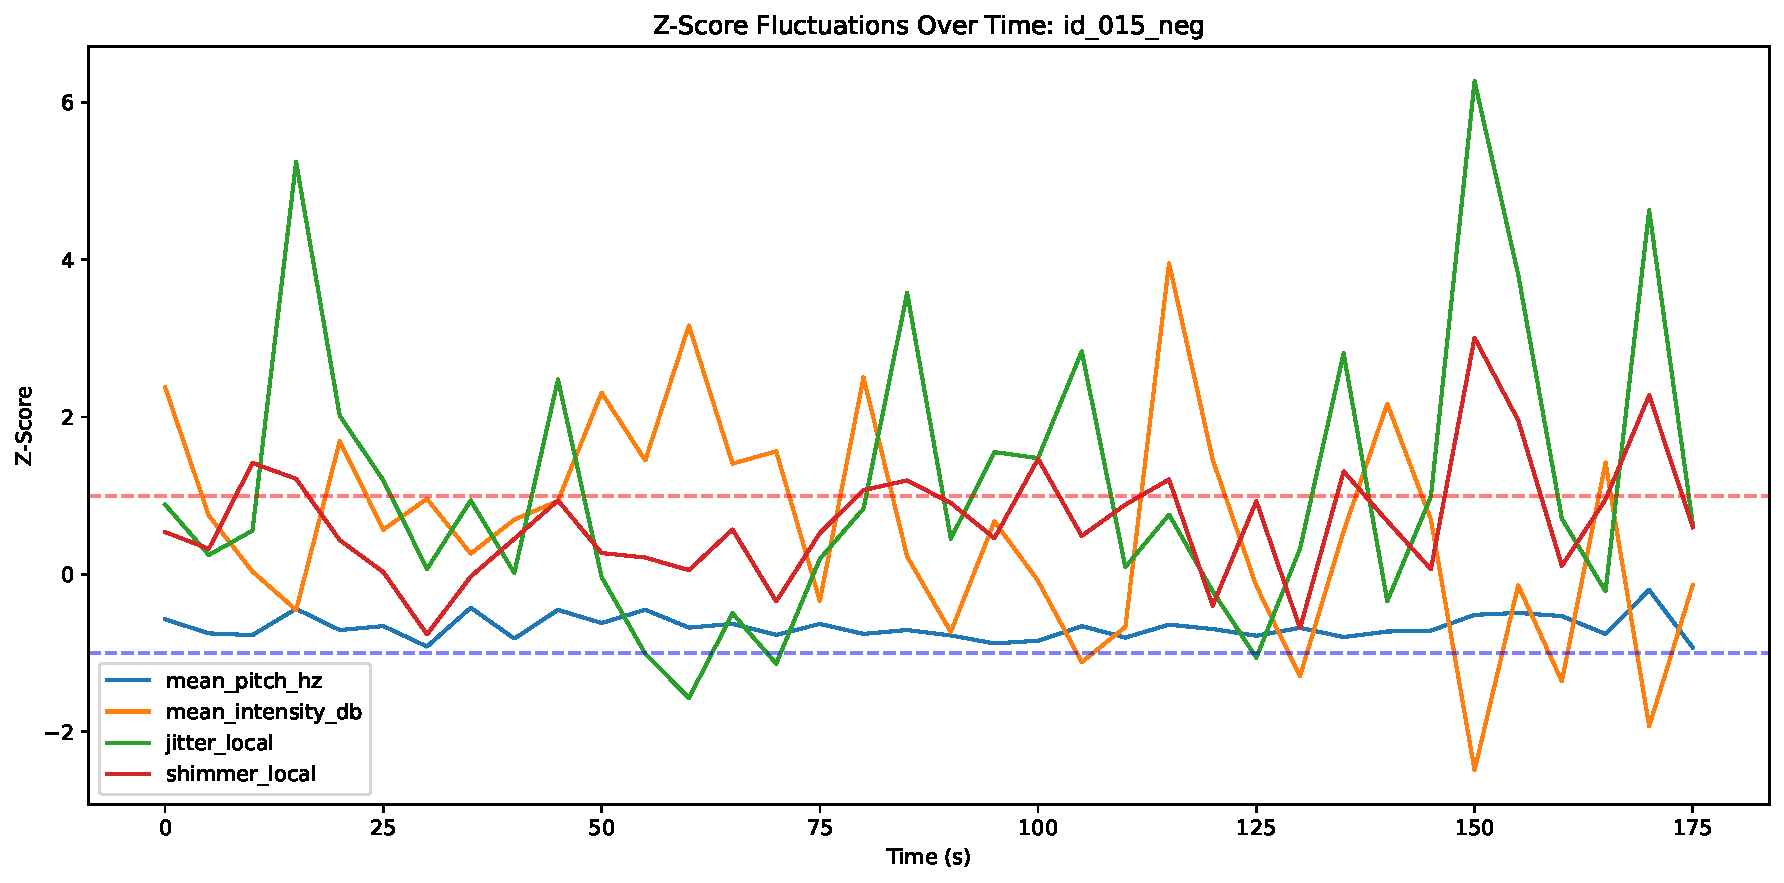
\includegraphics[width=0.7\textwidth]{png/results/rq1/zscore_fluctuations_id_015_neg.pdf}
    \caption{Z-score}
    \label{fig:z-score-15}
\end{figure}

\subsubsection{Summery}
This supports the idea that analyzing how vocal features change over time  can provide more meaningful insights into emotional expression in conversational, partly spontaneous speech during interviews compared to only using overall clip-level statistics.

\subsection{Conclusion RQ1 Data Analysis}
The results revealed only weak to moderate correlations for the analysis between individual vocal features and how Hume AI predicted emotions, where intensity and pitch showed most patterns consistently. 
The custom vocal categorization method did not function well in this context and resulted in very uniform results. This method was built on a basic group of vocal features which may overlooked important indicators for certain emotions. 
ANOVA tests found no significant differences in vocal features across AI-labeled emotions. However, examining pitch and intensity fluctuations over time segments in individual clips gave more promising results. This implies that dynamic changes in vocal features 
can offer more insights than static averages when analysing conversational, yet spontaneous speech during interviews. 

%%%%%%%%%%%%%%%%%%%%%%%%%%%%%%%%%%%%%%%%%%%%%%%%%%%%%%%%%%%%%%%%%%%%%%%%%%%%%%%%%%%%%%%%%%
                        %%%%%%%%%%%% RQ2 %%%%%%%%%%%%%%%%%%
 %%%%%%%%%%%%%%%%%%%%%%%%%%%%%%%%%%%%%%%%%%%%%%%%%%%%%%%%%%%%%%%%%%%%%%%%%%%%%%%%%%%%%%%%%%
\section{Data Analysis for RQ2: Text and Speech Based Emotion Recognition}
Research Question 2 explores the degree to which two modalities for AI-based emotion recognition systems - speech-based (Hume AI) and text-based (NLP Cloud) - agree or diverge when labelling emotional expressions in semi-structured interviews. 
We examine five target emotions (anger, joy, sadness, fear, surprise) across the full dataset, as well as positive and negative interviews separately. To acquire a detailed picture of how the models align, we compare their average emotion scores, 
measure Pearson correlations and paired t-tests with Cohen’s d. This multimethod approach supports a comprehensive understanding of how the two modalities responds to the same emotional input, to find mutual strengths and diverse tendencies in how they classify emotions. 
\subsection{Comparative Overview of Model Outputs}

As presented in Table~\ref{tab:rq3_emotion-stats-combined}, Table~\ref{tab:rq3_emotion-stats-pos}, and Table~\ref{tab:rq3_emotion-stats_neg} (\ref{sec:datacoll_rq2_rq3} Data Collection),
the mean emotion scores and standard deviations differ between the two models across the full dataset,
including patterns within positive and negative interviews. 

Figure \ref{fig:rq2_sent_grouped_bar} visualises these differences for positive and negatives recordings separately. As presented, anger in positive interviews was detected as significantly higher levels by Hume compared to NLP, 
that rated anger near zero. For the negative interviews, the rating was more aligned where NLP rated anger slightly higher. Joy is rates substantially high by NLP in the positive interviews, compared to both other emotions and Hume’s probability. 
In contrast, Hume rates joy higher than NLP for negative recordings. Sadness and fear are both rated higher by Hume than NLP in positive contexts, while NLP rates sadness higher in negative contexts where fear has more aligned scoring by the systems. 
Surprise was detected at similar, low levels by both models for both sentiment categories. 
Highest contrast for surprise is found in positive interviews where NLP rated it slightly higher.  

\begin{figure}[!h]
    \centering 
    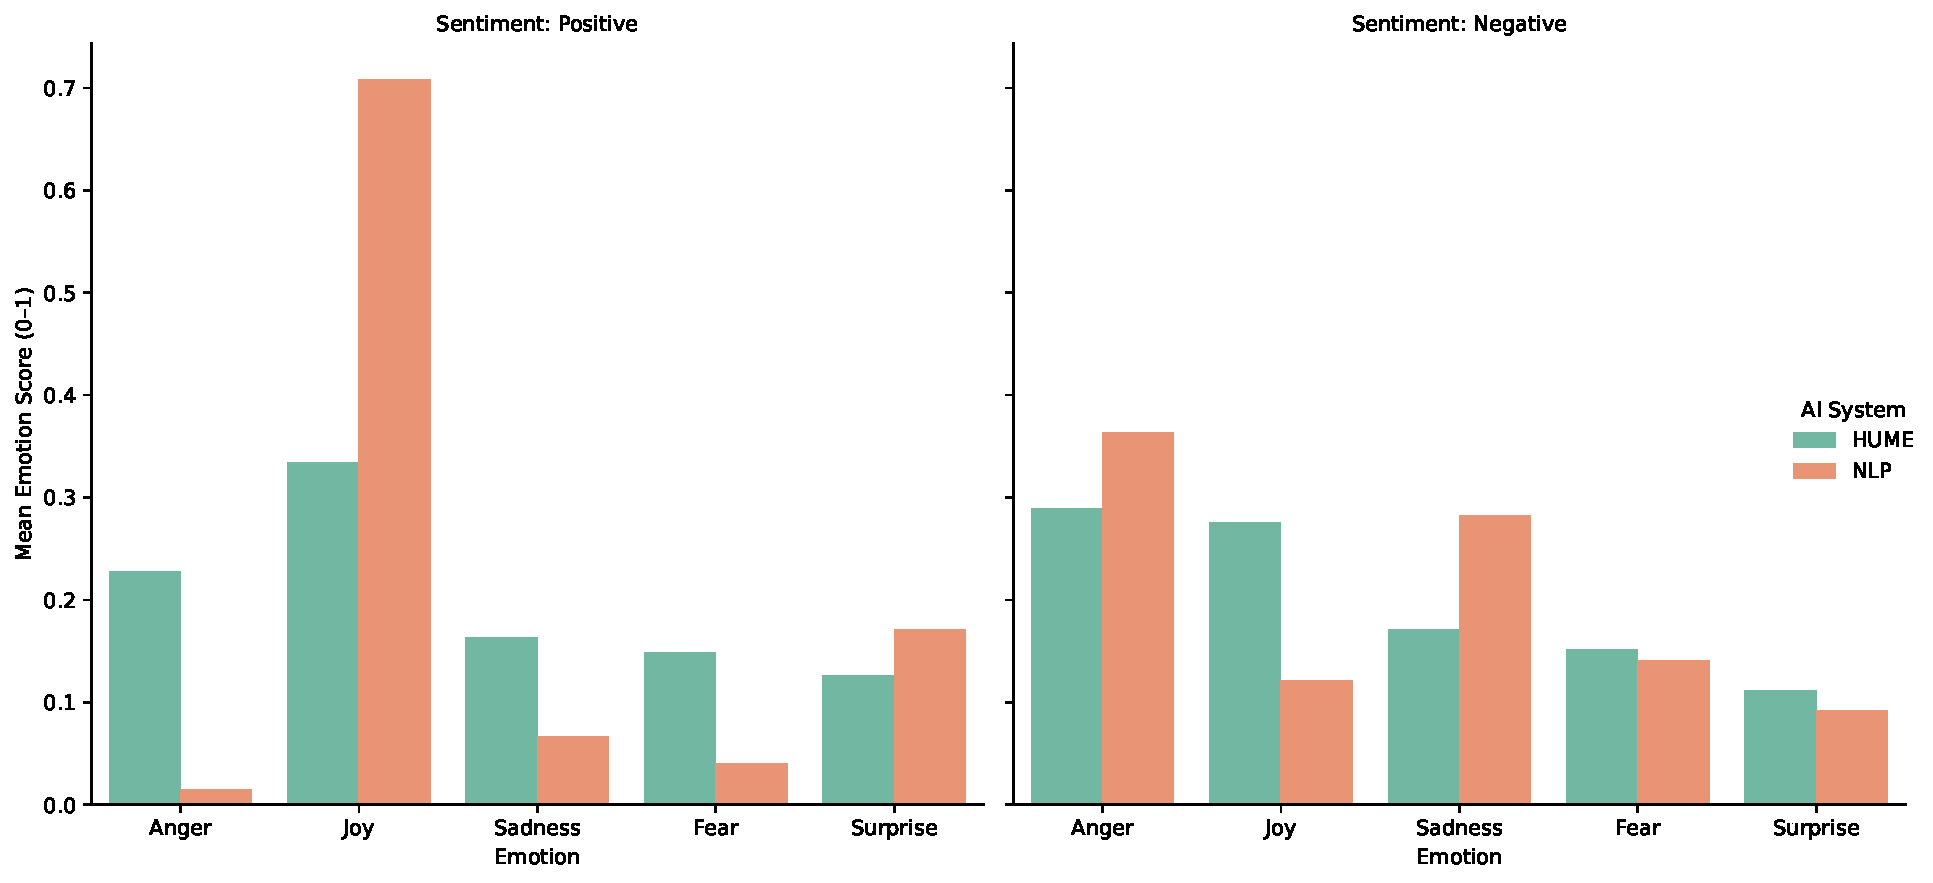
\includegraphics[width=0.95\textwidth]{png/results/rq2/sentiment_comparison_facet_all.pdf}
    \caption{Average emotion score for Hume AI and NLP Cloud, seperated by positive and negative recordnigs.}
    \label{fig:rq2_sent_grouped_bar}
\end{figure}

The differences in the average emotion scoring are presented further in Figure \ref{fig:rq2_avg_diff_full}. Positive values indicate that Hume AI assigned higher scores for respective emotions, while negative values imply higher scores from NLP Cloud. 
As explained for Figure \ref{fig:rq2_sent_grouped_bar}, the most evident difference was shown for joy in both sentiment contexts, where NLP rates it significantly higher in positive settings and Hume higher in negative settings. 
Differences for sadness and surprise were insignificant in negative interviews, aligned with surprise in positive interviews. 
In Figure \ref{fig:rq2_avg_diff_full}, the divergence in rating of fear in negative contexts is obvious where NLP rated the emotion more frequent. 

\begin{figure}[!h]
    \centering 
    \begin{subfigure}[b]{0.49\textwidth}
        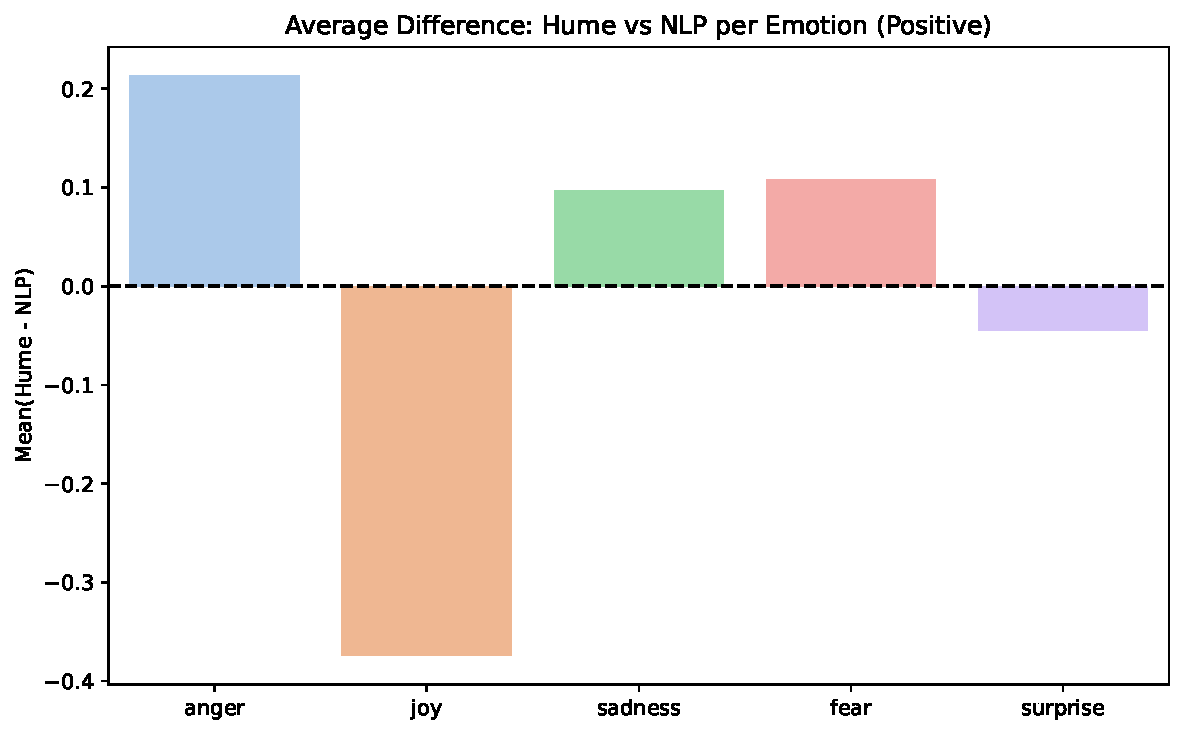
\includegraphics[width=\textwidth]{png/results/rq2/hume_nlp_difference_positive.pdf}
        \caption{Positive recordings.}
        \label{fig:rq2_avg_diff_pos}
    \end{subfigure}
    \begin{subfigure}[b]{0.49\textwidth}
    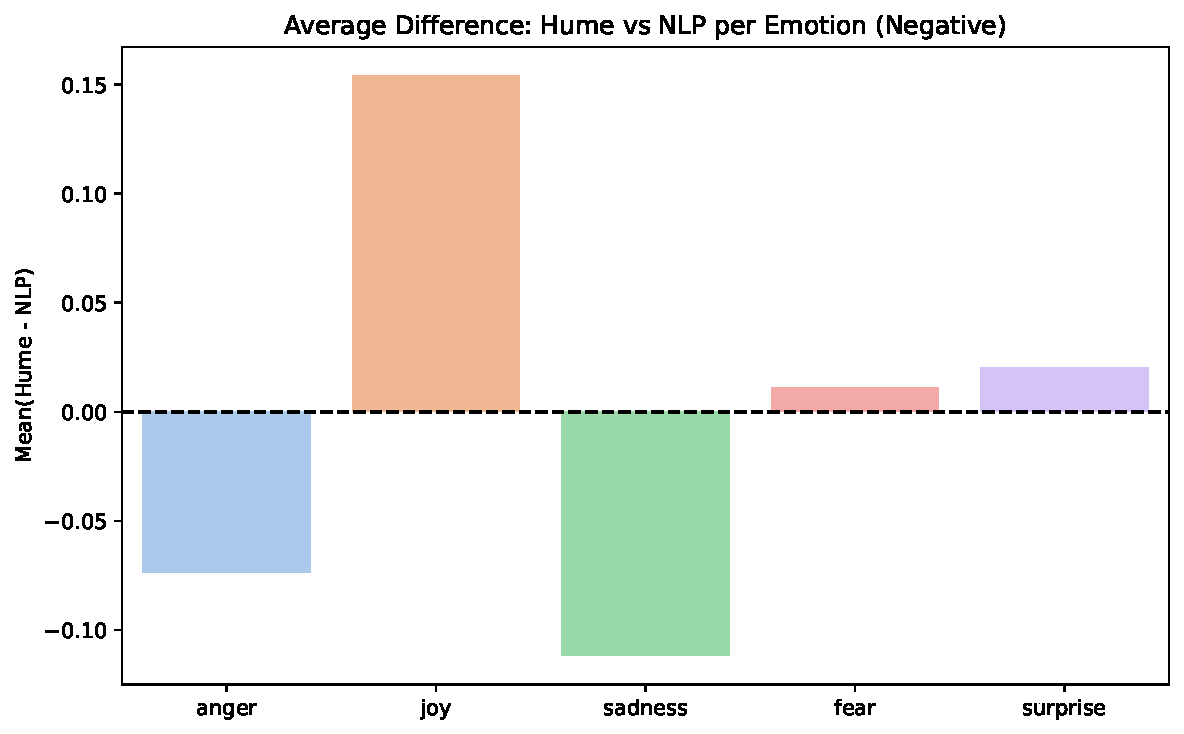
\includegraphics[width=\textwidth]{png/results/rq2/hume_nlp_difference_negative.pdf}
    \caption{Negative recordings.}
    \label{fig:rq2_avg_diff_neg}
    \end{subfigure}
    \caption{Average difference in emotions scores between Hume and NLP.}
    \label{fig:rq2_avg_diff_full}
\end{figure}

\newpage
\subsection{Statistical Analysis}
\subsubsection{Correlation Analysis}

To evaluate how text-based (NLP Cloud) and speech-based (Hume AI) emotion recognition aligns, Pearson correlation coefficients (r) were calculated for each emotion across all interview recordings. 
Table~\ref{tab:corr_all} includes the full dataset (positive and negative recordings), presenting the correlation values as well as corresponding p-values to examine the statistical significance. 

\begin{table}[H]
    \centering
    \caption*{\textbf{All recordings}}
    \begin{tabular}{lrrl}
      \toprule
      \textbf{Emotion} & \textbf{Pearson r} & \textbf{p-value} & \textbf{Significant}\\
      \midrule
      Anger    & 0.466 & 0.007 & Yes \\
      Joy      & 0.521 & 0.002 & Yes \\
      Sadness  & 0.167 & 0.362 & No  \\
      Fear     & 0.171 & 0.348 & No  \\
      Surprise & 0.197 & 0.281 & No  \\
      \bottomrule
    \end{tabular}
    \caption{Pearson Correlations Between NLP and Hume Emotion Scores (Full dataset)}
    \label{tab:corr_all}
  \end{table}

This data demonstrates a reasonable positive correlation for Anger(r = 0.466, p=0.007) and Joy (r=0.521, p=0.0022), implying that these emotions are relatively consistent identified throughout the AI systems on the full dataset. 
The p-values (p<0.05) show a statistical significance and highlights a relevant relationship in how Anger and Joy are detected through different processes. 
Sadness, Fear, and Surprise show contrasted results with weak correlations (r<0.20) where the p-values indicate no significancy with low agreement between the AI models for these emotions when analysing the full dataset. 
Overall, some alignment for the more distinct emotions as Anger and Joy are declared through the correlation analysis, but some difficulties with consistent agreement are prominent for more nuances emotions as Sadness, Fear, and Surprise. 

\begin{table}[H]
    \centering
    \caption*{\textbf{Positive Recordings}}
    \begin{tabular}{lrrl}
      \toprule
      \textbf{Emotion} & \textbf{Pearson r} & \textbf{p-value} & \textbf{Significant}\\
      \midrule
      Anger    & 0.160  & 0.568 & No  \\
      Joy      & 0.682  & 0.005 & Yes \\
      Sadness  & 0.546  & 0.035 & Yes \\
      Fear     & 0.098  & 0.729 & No  \\
      Surprise & -0.050 & 0.860 & No  \\
      \bottomrule
    \end{tabular}
    \caption{Pearson Correlations Between NLP and Hume Emotion Scores (Positive)}
    \label{tab:corr_pos}
  \end{table}
Table \ref{tab:corr_pos} presents the same data as Table \ref{tab:corr_all}, but for positive recordings separately. As for the full dataset, Joy shows a significant correlation (r = 0.682, p = 0.005) between the model’s detection. In contrast, Anger has a lower correlation (r = 0.160, p = 0.568) in positive contexts and Sadness presents a significant correlation (r = 0.549, 0.035) distinct from the full dataset. Fear and Surprise has even lower correlations for positive recordings than the dataset combined, with p-values close to 1. 

\begin{table}[H]
    \centering
    \caption*{\textbf{Negative Recordings}}
    \begin{tabular}{lrrl}
      \toprule
      \textbf{Emotion} & \textbf{Pearson r} & \textbf{p-value} & \textbf{Significant}\\
      \midrule
      Anger    & 0.260 & 0.313 & No  \\
      Joy      & 0.556 & 0.020 & Yes \\
      Sadness  & 0.028 & 0.914 & No  \\
      Fear     & 0.270 & 0.294 & No  \\
      Surprise & 0.209 & 0.422 & No  \\
      \bottomrule
    \end{tabular}
    \caption{Pearson Correlations Between NLP and Hume Emotion Scores (Negative)}
    \label{tab:corr_neg}
  \end{table}
  Table \ref{tab:corr_neg} summerizes the correlation coefficients for the negative recordings. Consistent with the full dataset and positive subset, Joy again demonstrated  a significant correlation in negative contexts (r = 0.556, p = 0.020). 
  All other emotions failed to reach significance, with values that markedly diverged from their corresponding values in the positive recordings: 
  Sadness resulted r = 0.028 (p = 0.914) versus r = 0.546 (p = 0.035) for positives, and Fear showed r = 0.270 (p = 0.294) compared to r = 0.098 (p = 0.729) in the positive context. 



\subsubsection{Paired t-Tests and Effect Sizes}
To further explore alignment and differences between speech-based (Hume AI) and text-based (NLP Cloud) emotion recognition, paired t-tests and Cohen's d were conducted. 
Table \ref{tab:t-test-all} shows the t-statistics, p-values, and Cohen's d for each emotion across the full dataset. Positive t-values implies that Hume rated that emotion more frequent than NLP, negative t-values suggest the opposite.

\begin{table}[H]
    \centering
    \caption*{\textbf{Full Dataset}}
    \begin{tabular}{lrrlr}
      \toprule
      \textbf{Emotion} & \textbf{t‐statistic} & \textbf{p‐value} & \textbf{Significant} & \textbf{Cohen’s d} \\
      \midrule
      Anger    &  1.717 & 0.096  & No  &  0.303 \\
      Joy      & -1.726 & 0.094  & No  & -0.305 \\
      Sadness  & -0.548 & 0.588  & No  & -0.097 \\
      Fear     &  3.341 & 0.002  & Yes &  0.591 \\
      Surprise & -0.657 & 0.516  & No  & -0.116 \\
      \bottomrule
    \end{tabular}
    \caption{t‐statistics, p‐value with significance, and Cohen’s d for all clips.}
    \label{tab:t-test-all}
\end{table}
Across all interviews, only Fear had statistically significant difference between the AI-models (t = 3.341, p = 0.0022), and had a medium effect size (Cohen's d = 0.591).
Hume AI rated fear consistently higher than NLP Cloud, suggesting a systematic modality difference for this emotion. 
Although Anger, Joy, Sadness, and Surprise had some mean-score differences, none reached statistical significance (all p>0.05) and their effect sizes were small (|d| < 0.03). 
Apart from Fear, the two models demonstrated close agreement in recognizing these emotional expressions. 

\begin{table}[H]
    \centering
    \caption*{\textbf{Positive Recordings}}
    \begin{tabular}{lrrlr}
      \toprule
      \textbf{Emotion} & \textbf{t‐statistic} & \textbf{p‐value} & \textbf{Significant} & \textbf{Cohen's d} \\
      \midrule
      Anger    & 10.903  & 0       & Yes & 2.815  \\
      Joy      & -11.665 & 0       & Yes & -3.012 \\
      Sadness  & 6.177   & 0       & Yes & 1.595  \\
      Fear     & 5.125   & 0       & Yes & 1.323  \\
      Surprise & -1.723  & 0.107   & No  & -0.445 \\
      \bottomrule
    \end{tabular}
    \caption{t‐statistics, p‐value with significance, and Cohen's d for positive interviews.}
    \label{tab:t-test-pos}
\end{table}
Table \ref{tab:t-test-pos} demonstrates t-tests and Cohen's d for positive oriented interviews, where all emotions except for surprise (t = -1.723, p = 0.107, d = -0.445) shows significant differences (p < 0.001)
with certainly large effect sizes. Negative T-value and Cohen's d for Joy (t = -11.665, d = -3.012) indicates that NLP have the aspects of overestimating this emotion compared to Hume with large effect sizes, where Hume in contrast tends to overestimate Anger (t = 10.903, d = 2.815) in positive contexts. 
Hume rates Sadness and Fear more prominent than NLP, and Surprise remain inconsistent as previous results with no significant difference (t = -1.723, p = 0.107). 

\begin{table}[H]
    \centering
    \caption*{\textbf{Negative Recordings}}
    \begin{tabular}{lrrlr}
      \toprule
      \textbf{Emotion} & \textbf{t-statistic} & \textbf{p-value} & \textbf{Significant} & \textbf{Cohen’s d} \\
      \midrule
      Anger    & -1.702 & 0.108   & No  & -0.413 \\
      Joy      &  3.720 & 0.002   & Yes &  0.902 \\
      Sadness  & -3.796 & 0.002   & Yes & -0.921 \\
      Fear     &  0.536 & 0.599   & No  &  0.130 \\
      Surprise &  1.311 & 0.208   & No  &  0.318 \\
      \bottomrule
    \end{tabular}
    \caption{t-statistics, p-value with significance, and2 Cohen’s d for negative interviews.}
    \label{tab:t-test-neg}
  \end{table}
Table \ref{tab:t-test-neg} presents conducted t-tests and Cohen's d in negative interviews, with significant differences for Joy (t = 3.720, p = 0.002), where Hume rates it significantly higher than NLP. 
In contrast, NLP has clear higher scoring for Sadness with large effect size (t = -3.796, d = -0.921). However, the effect sizes are not as big as for the positive recordings. 
For example, the effect sizes for Joy (t = 0.902) are lower than Joy in positive contexts (t = -3.012) where NLP overestimated the emotion compared to Hume.
Anger has a moderate difference, even if it is not statistically significant. No notable differences are detected for either Fear or Surprise. 
This implies that the AI systems strongly disagrees on Joy and Sadness detection in the negative contexts of the dataset. 

\subsubsection{Conclusion Statistical Analysis}
Comparison of speech-based (Hume AI) and text-based (NLP Cloud) with statistical analysis demonstrates correlation particularly for clear expressed emotions as Anger and Joy when analysing the full dataset. 
However, anger shows no correlation between the models for either positive or negative recordings when separated. Joy shows a significant correlation throughout all sentiment contexts, 
where t-tests confirmed that NLP had higher predictions for joy in positive contexts and Hume in negative. 
Emotions that are more subtle like Sadness, Fear, and Surprise, revealed low correlations for all sentiment contexts except positive that showed a strong correlation for sadness, indicating modality-specific distinctions. 
Paired t-tests strengthened this observation regarding the full dataset and negative subset, pointing out Fear as the only emotion with statistically significant divergence in the full dataset where speech-based analysis assigned higher scores consistently. 
However, negative recordings showed significant difference for joy and sadness, while positively oriented clips showed significant difference for all emotions except surprise. 







\subsubsection{Conclusion Sentiment-Based Analysis}
In conclusion, Hume AI and NLP Cloud show moderate to strong agreement on anger (r = 0.47) and joy (r = 0.52) across the full dataset, but weak correlations on sadness, fear, and surprise. Paired t-tests showed that fear is the single emotion that exhibits a significant mean difference across the full interview set (Hume > NLP, d = 0.59), while joy and anger showed modality divergencies in positive and negative subsets where NLP overestimated joy in positive interviews (d = 3.01) and Hume overestimated anger (d = 2.82). These results suggest that text and speech modalities agree on certain emotions particularly when considering the full dataset. However, divergencies occur for sentiment-specific analyses, especially for positive interviews. 

\subsubsection{Case Example}
single clip comparison 

breifly illustrate how speech vs text differ in practice 

\subsection{Conclusion of RQ2 Data Analysis}
The results of this research question show that even if Hume AI and NLP Cloud partially aligns in detecting emotions, certainly for clearly expressed emotions such as Anger and Joy, 
they diverge significantly in their predictions of more nuanced emotions such as Fear, Sadness, and Surprise. Statistical tests confirmed a significant difference for Fear. 
Sentiment-based analysis showed that emotional context have an impact on the results, when analysing five basic emotions, where positive scenarios had a larger model divergence. 
As discussed above, the interview setting and overall data collection may have different impacts on the results. Still, the findings highlights how speech- and text-based models are complementary, each 
with their own strenghts to capture different aspects of emotion expression, and indicate that relying on a single modality could have limitations for comprehensive emotion detection in speech.  


%%%%%%%%%%%%%%%%%%%%%%%%%%%%%%%%%%%%%%%%%%%%%%%%%%%%%%%%%%%%%%%%%%%%%%%%%%%%%%%%%%%%%%%%%%
                        %%%%%%%%%%%%%%%%%%%%% RQ3   %%%%%%%%%%%%%%%
%%%%%%%%%%%%%%%%%%%%%%%%%%%%%%%%%%%%%%%%%%%%%%%%%%%%%%%%%%%%%%%%%%%%%%%%%%%%%%%%%%%%%%%%%%
\section{Data Analysis for RQ3: AI and self-assessed emotion labels}

The third research question explores how AI-generated emotion labels - from both speech-based (Hume AI) and text-based (NLP Cloud) 
analyses - aligns with self-assessed emotions. It is of importance to understand how these AI systems reflect humans perception of 
their own emotions and explore how the systems align with the participants own emotional viewpoint.  
To answer this question, participants own assessments are compared with AI-labels to gain an understanding if these systems are aligned with human self-perception of their emotions and how the modality affects the results. 
To explore alignment and divergence, the analysis include comparisons of average scoring, correlations, statistical analysis, and sentiment separation.  
\subsection{Model Emotion Score and Self-Reports Comparison}

An initial overview is summarised in Table~\ref{tab:rq3_emotion-stats-combined}, Table~\ref{tab:rq3_emotion-stats-pos}, and Table~\ref{tab:rq3_emotion-stats_neg} (\ref{sec:datacoll_rq2_rq3} Data Collection),
with average emotion scores across all 30 interview recordings for each emotion category (anger, joy, sadness, fear, surprise). The table presents mean values and standard deviation for self-resported scores 
aside both AI-systems.Table~\ref{tab:rq3_emotion-stats-pos} includes the same values for positive recordings and Table~\ref{tab:rq3_emotion-stats_neg} presents the data from negative recordings.

These differences are visualized in Figure~\ref{fig:comp-bar-rq3-all}, illustrating a bar chart that compares the average emotion scores defined by 
Hume AI, NLP Cloud, and participants self-assessment seperated by positive and negative oriented interviews.

\begin{figure}[!h]
    \centering
    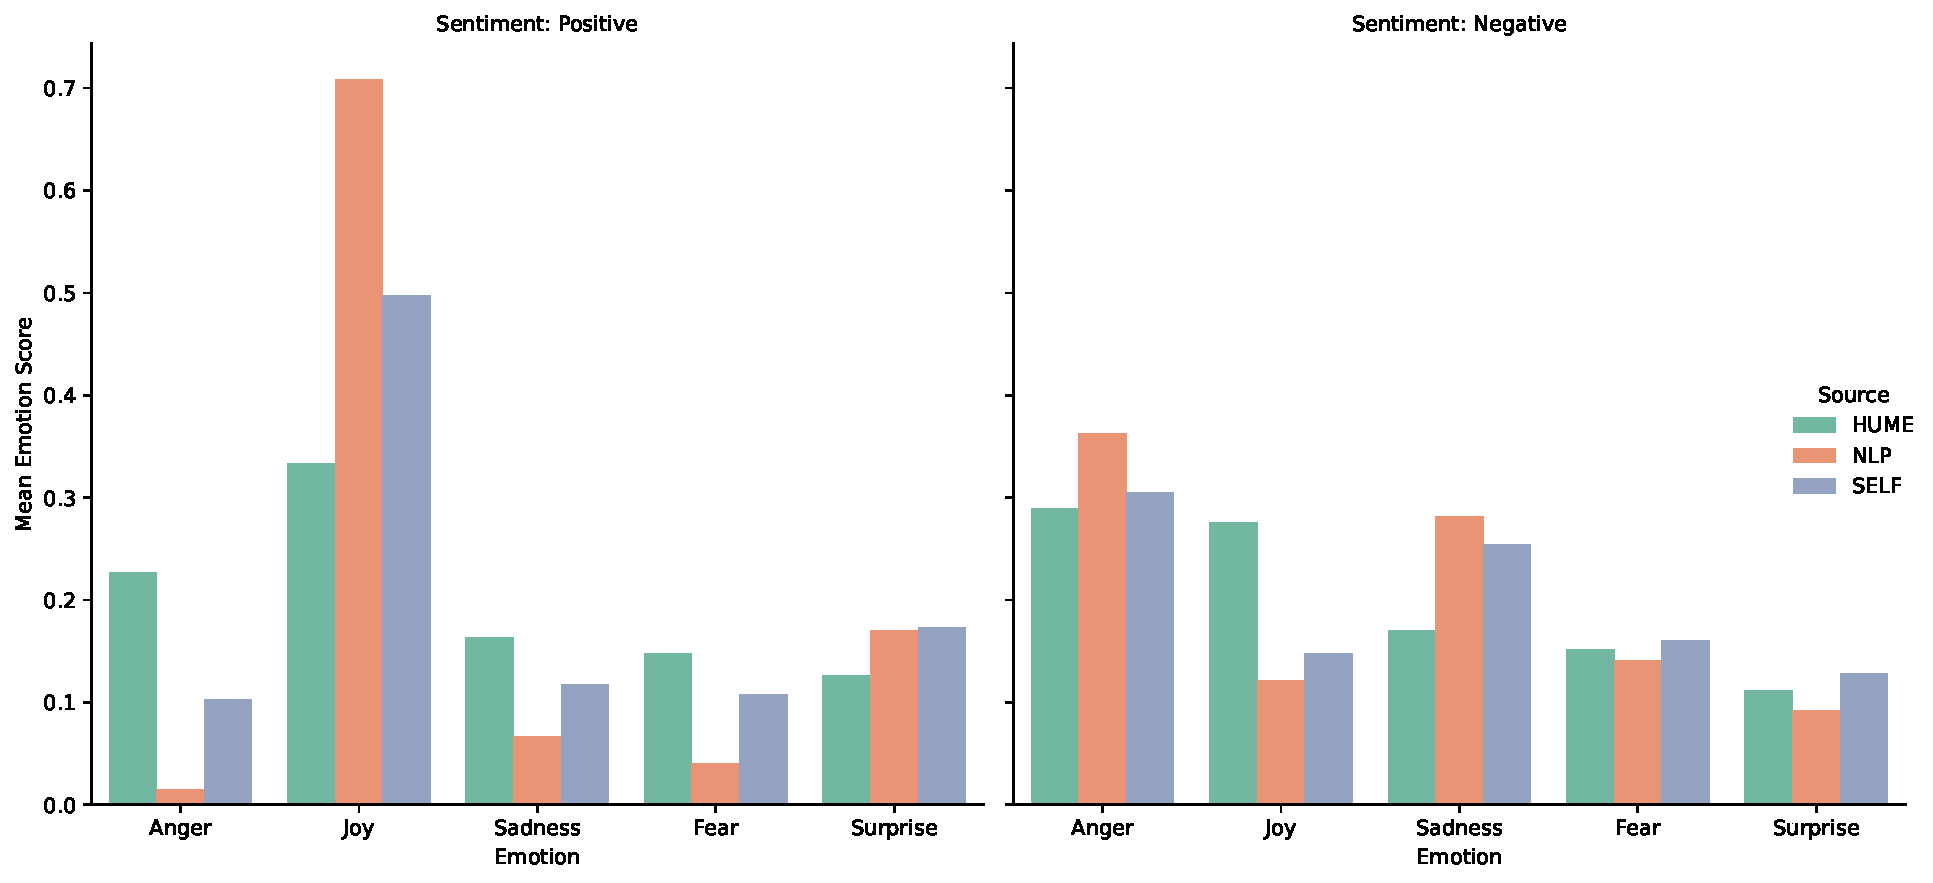
\includegraphics[width=0.95\textwidth]{png/results/rq3/rq3_sentiment_grouped_bar.pdf}
    \caption{Comparison of emotional labels for Hume, NLP, and self-assessed.}
    \label{fig:comp-bar-rq3-all}
\end{figure}

For the positive recordings, Joy consistently had higher self-reported scores than other emotions. NLP rates Joy higher than the participants while Hume rates it lower. 
In contrast, Joy was markedly rated higher by Hume in negative contexts than NLP and self-reporting which rated the emotion equally. The negative related emotions (Anger, Sadness, Fear) were assessed at lower levels by participants in the positive interviews. 
Self-assessed scores generally matched Hume’s higher detection of Sadness, Fear and Surprise than NLP’s minor predictions. Anger had higher rating by Hume than both self-reports and NLP in positive contexts. 
Surprise had similar average score across all sources, slightly lower detection rate by Hume. 

For negative recordings, Anger had similar rating across all sources, with slightly higher rating by NLP.  Joy has markedly higher average score by Hume compared to the other sources, while the speech-model rates Sadness lower than the text-model and participants. 
Fear and surprise had aligned rating by all sources, with a similar pattern where both emotions are rated slightly higher by the participants, closely followed by Hume and lowest rating by NLP. 

This comparison suggests that emotional ranking are more aligned in for the negative recordings, where Joy is the emotion most distinct in the rating by Hume. 
The positive oriented interviews have more varying results between the sources, Joy are significanly rated higher by NLP while the text-based model rates Anger close to zero compared to Hume that rates this emotion higher than all other emotions except for Joy. 

The sentiment-based comparison clearly presents that emotional expression and self-awareness have a signficant variance between modalities and emotional contexts. 
Explicit emotions articulated in words are closely aligned between self-assessed rating and text-based analysis. 
While implicit or suble emotions expressed through vocal tone have a notable divergence. 

\subsection{Correlation and Visual Analysis}
To evaluate the alignment between AI-generated emotion scores and participants self-reported emotions, 
Pearson correlation analyses were conducted across the five emotion categories for both speech-based (Hume AI) and text-based (NLP Cloud) compared to self-reporting.
With these measurements the relationship's strength and direction and the statistical significance can be reviewed. 

\subsubsection{Hume AI vs Self-Reported Emotions}
%%% Correlation hume self 
\begin{table}[H]
    \centering
    \caption*{\textbf{All Hume}}
    \begin{tabular}{lrrl}
      \toprule
      \textbf{Emotion} & \textbf{Pearson’s \(r\)} & \textbf{\(p\)-value} & \textbf{Significant} \\
      \midrule
      Anger    & 0,359 & 0,043 & Yes \\
      Joy      & 0,334 & 0,062 & No  \\
      Sadness  & 0,050 & 0,784 & No  \\
      Fear     & \(-\)0,007 & 0,969 & No  \\
      Surprise & 0,088 & 0,631 & No  \\
      \bottomrule
    \end{tabular}
    \caption{Pearson’s \(r\), \(p\)-values, and significance for all Hume recordings.}
    \label{tab:rq3_corr-hume-all}
  \end{table}

The correlation results for Hume AI predictions on all recordings in the dataset is demonstrated in Table~\ref{tab:rq3_corr-hume-all}, and indicate generally weak correlations across the majority of emotions. 
Anger is the only emotion showing a statistic significant correlation (r = 0.359, p = 0.043), which indicates a moderate alignment between Hume AI's speech based emotion 
detection and participants own perception for this emotion. Joy shows a moderate correlation but without statistical significance (r = 0.334, p = 0.062), other emotions, such as Fear (r = 0.007, p = 0.969), presents no relevant correlation. 

  \begin{table}[H]
    \centering
    \caption*{\textbf{Positive Recordings (Hume)}}
    \begin{tabular}{lrrl}
      \toprule
      \textbf{Emotion} & \textbf{Pearson’s \(r\)} & \textbf{\(p\)-value} & \textbf{Significant} \\
      \midrule
      Anger    & 0,404 & 0,136 & No  \\
      Joy      & 0,401 & 0,138 & No  \\
      Sadness  & 0,320 & 0,244 & No  \\
      Fear     & \(-\)0,027 & 0,924 & No  \\
      Surprise & 0,091 & 0,748 & No  \\
      \bottomrule
    \end{tabular}
    \caption{Pearson’s \(r\), \(p\)-values, and significance for positive recordings.}
    \label{tab:rq3_corr-hume-pos}
  \end{table}

  Table \ref{tab:rq3_corr-hume-pos} presents correlation coefficients for positive recordings with no significant agreement occurs between Hume predictions and self-reported emotions. Anger, sadness, and sadness show moderate correlations (r = 0.320-0.404) with no statistical significance (p = 0.136-0.244). Weak correlation appears for both fear and surprise with high p-values suggesting no convincing evidence for these correlations. 

  \begin{table}[H]
    \centering
    \caption*{\textbf{Negative Recordings (Hume)}}
    \begin{tabular}{lrrl}
      \toprule
      \textbf{Emotion} & \textbf{Pearson’s \(r\)} & \textbf{\(p\)-value} & \textbf{Significant} \\
      \midrule
      Anger    & \(-\)0,105 & 0,690 & No  \\
      Joy      & 0,127     & 0,627 & No  \\
      Sadness  & \(-\)0,146 & 0,576 & No  \\
      Fear     & \(-\)0,036 & 0,891 & No  \\
      Surprise & \(-\)0,143 & 0,585 & No  \\
      \bottomrule
    \end{tabular}
    \caption{Pearson’s \(r\), \(p\)-values, and significance for negative recordings.}
    \label{tab:rq3_corr-hume-neg}
  \end{table}

  Negatively oriented interviews are presented in Table~\ref{tab:rq3_corr-hume-neg} with similar results as for positive interviews where no correlations of significance are found (r = -0.146-0.127, p = 0.576-0.0.891). Four out of five emotion correlations are negative while joy has a weak positive relationship. Each correlation is considered weak without statistical significance, implying that Hume predicted emotions distinct from participants own evaluation.  
%%% Self vs NLP 
\subsubsection{NLP Cloud vs Self-Reported Emotions}
\label{sec:nlp-self}
\begin{table}[H]
    \centering
    \caption*{\textbf{All NLP}}
    \begin{tabular}{lrrl}
      \toprule
      \textbf{Emotion} & \textbf{Pearson’s \(r\)} & \textbf{\(p\)-value} & \textbf{Significant} \\
      \midrule
      Anger    & 0,739 & 0,000 & Yes \\
      Joy      & 0,863 & 0,000 & Yes \\
      Sadness  & 0,710 & 0,000 & Yes \\
      Fear     & 0,669 & 0,000 & Yes \\
      Surprise & 0,092 & 0,616 & No  \\
      \bottomrule
    \end{tabular}
    \caption{Pearson’s \(r\), \(p\)-values, and significance for all NLP recordings.}
    \label{tab:rq3_corr-nlp-all}
  \end{table}

  Table \ref{tab:rq3_corr-nlp-all} presents correlation coefficients between self-reported and NLP-predicted emotions for the full dataset.
  When analysing the full dataset, NLP Cloud demonstrated strong and statistically significant correlations with self-reporting for four of five emotions. Joy showed the strongest correlation (r = 0.863, p < 0.001), followed by Anger (r = 0.739, p < 0.001) and Sadness (r = 0.710, p < 0.001). 
Fear had a moderately strong correlation with high statistical significance (r = 0.669, p < 0.001). Surprise was the single emotion showing weak correlation with no statistical significance (r = 0.092, p = 616). 
  
  \begin{table}[H]
    \centering
    \caption*{\textbf{Positive Recordings (NLP)}}
    \begin{tabular}{lrrl}
      \toprule
      \textbf{Emotion} & \textbf{Pearson’s \(r\)} & \textbf{\(p\)-value} & \textbf{Significant} \\
      \midrule
      Anger    & \(-\)0,199 & 0,477 & No  \\
      Joy      & 0,622     & 0,013 & Yes \\
      Sadness  & 0,363     & 0,183 & No  \\
      Fear     & 0,527     & 0,043 & Yes \\
      Surprise & 0,011     & 0,969 & No  \\
      \bottomrule
    \end{tabular}
    \caption{Pearson’s \(r\), \(p\)-values, and significance for positive recordings (NLP).}
    \label{tab:rq3_corr-nlp-pos}
  \end{table}
  
  Table \ref{tab:rq3_corr-nlp-pos} presents correlation data between self-reports and NLP Cloud for positive interviews, where lower alignments between self-reports and NLP is found compared to the full dataset. 
  Only correlations for Joy (r = 0.622, p = 0.013) and Fear (r = 0.527, p = 0.043) are statistically significant. Sadness had a moderate correlation without statistical significance, Anger and Surprise presented weak correlations. 
  \begin{table}[H]
    \centering
    \caption*{\textbf{Negative Recordings (NLP)}}
    \begin{tabular}{lrrl}
      \toprule
      \textbf{Emotion} & \textbf{Pearson’s \(r\)} & \textbf{\(p\)-value} & \textbf{Significant} \\
      \midrule
      Anger    & 0,286     & 0,266 & No  \\
      Joy      & 0,366     & 0,149 & No  \\
      Sadness  & 0,429     & 0,086 & No  \\
      Fear     & 0,599     & 0,011 & Yes \\
      Surprise & \(-\)0,146 & 0,575 & No  \\
      \bottomrule
    \end{tabular}
    \caption{Pearson’s \(r\), \(p\)-values, and significance for negative recordings (NLP).}
    \label{tab:rq3_corr-nlp-neg}
  \end{table}
  
Table \ref{tab:rq3_corr-nlp-neg} demonstrates correlation coefficients for negative interviews, with similar results as for the positive interviews with weaker correlations compared to the full dataset. The single strong correlation with statistical significance is Fear (r = 0.599, p = 0.011). 
Moderate correlation is found for Joy (r = 0.366 p = 0.149) and Sadness (r = 0.429, p = 0.086), both with no statistical significance. As for the positive recordings, both Anger and Surprise had weak correlations between NLP and self-reporting. 


\subsubsection{Visual Correlation}
Figure \ref{fig:scatter-anger-rq3} illustrates the correlation between self-reported Anger scores and AI-labeled predictions. As shown, Hume AI shows a weak to moderate positive tendency (r = 0.36, p = 0.043), still reaches statistical significance, even if the data points are more dispersed around the trend line. 
In contrast, NLP Cloud shows a strong and statistical significant correlation (r = 0.74, p < 0.0001), which is visually very noticable with the tightly clustered linear relationship. 

%% ANGER
\begin{figure}[!h]
    \centering
    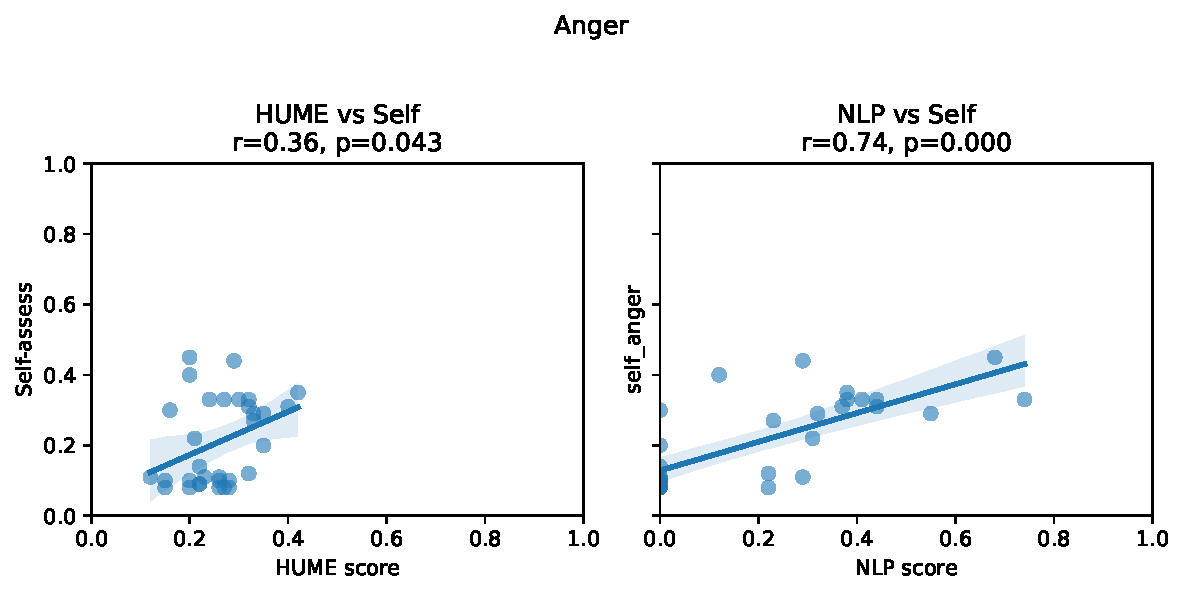
\includegraphics[width=0.7\textwidth]{png/results/rq3/scatter_anger_vs_self.pdf}
    \caption{Scatter plot, Hume, NLP vs. Self for Anger.}
    \label{fig:scatter-anger-rq3}
\end{figure}

Figure \ref{fig:scatter-joy-rq3} demonstrates the Joy correlation between self-reports and AI-predictions. Similar to Anger, Hume AI presents a weak to moderate positive trend (r = 0.33, p = 0.062), however it does not reach statistical significance. The diagram illustrates a disperse for the data points comparable to Anger.
As stated in previous results, NLP Cloud reveal a prominent statistical correlation (r = 0.86, p < 0001), clearly presented in the diagram. 
%% JOY
\begin{figure}[!h]
    \centering
    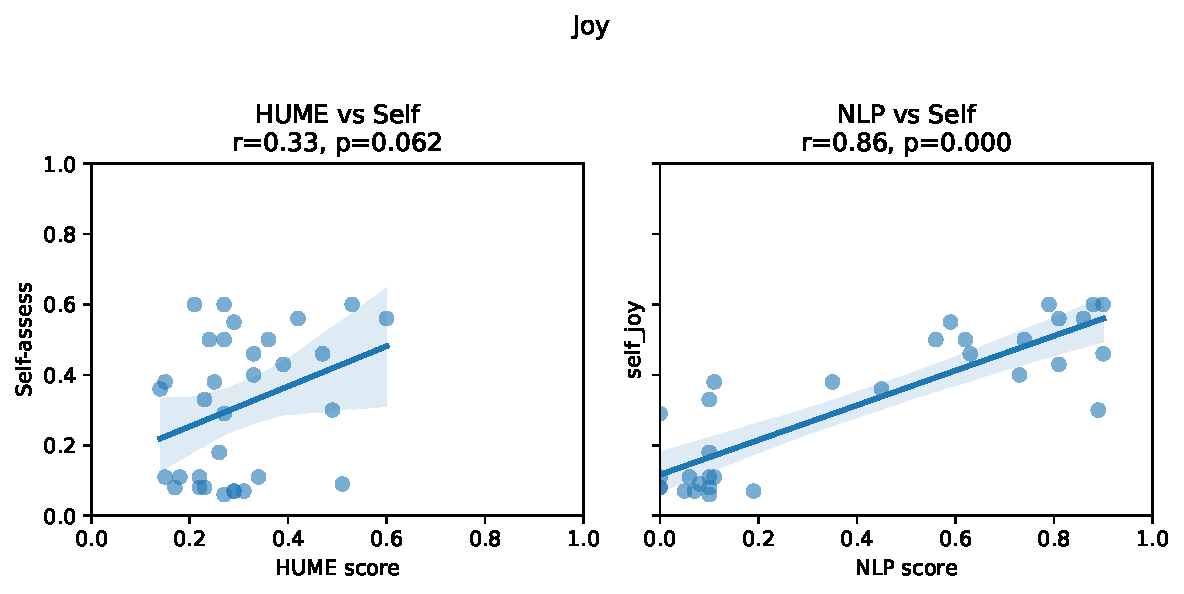
\includegraphics[width=0.7\textwidth]{png/results/rq3/scatter_joy_vs_self.pdf}
    \caption{Scatter plot, Hume, NLP vs. Self for Joy.}
    \label{fig:scatter-joy-rq3}
\end{figure}
\medskip

Figure \ref{fig:scatter-surprise-rq3} presents the correlation results for Surprise. Both Hume AI and NLP Cloud has minor correlation with self-reported Surprise scoring (r = 0.09), the lack of alignment is reflected in the scattered plots where no direct clear linear trend is shown. 
As stated in \ref{sec:rq2-sentiment} RQ2, Sentiment-Based Analysis, the inconsistent results may be due to Surprise being slighter expressed during the interviews. For this research question, it is important to note that several participants expressed confusion about how to interpret and answer 
their experienced Surprise, which can affect these inconsistent outcomes. 
%% SURPRISE 
\begin{figure}[!h]
    \centering
    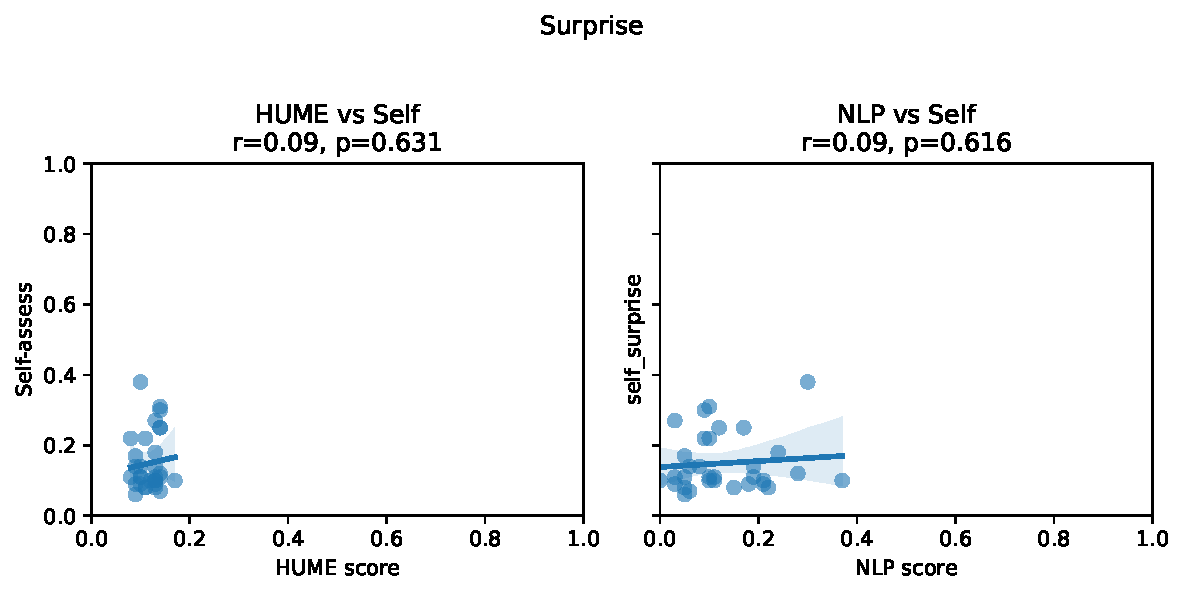
\includegraphics[width=0.7\textwidth]{png/results/rq3/scatter_surprise_vs_self.pdf}
    \caption{Scatter plot, Hume, NLP vs. Self for Surprise.}
    \label{fig:scatter-surprise-rq3}
\end{figure}

The scatter plots support previous presented statistical findings, highlighting the higher consistency of alignment between NLP Cloud and participant assessment for explicit expressed emotions as Joy and Anger. 
The shared difficulty of both models in detecting Surprise is presented further, possibly due to participant misunderstanding or that the interview scenarios were not oriented directly towards Surprise. 

\subsubsection{Conclusion Correlation and Visual Analysis}
This section reveal a clear trend, both statistically and visually: NLP Cloud aligns strongly with self-reported emotions for four out of five emotions, Anger, Joy, Sadness, and Fear, while Hume has weaker and 
non-significant correlations except for Anger. Both AI-models show weak levels of detecting Surprise, likely due to the interview setting and participant understanding of the question. 
These results emphasize the strength of text-based emotion analysis for recognition of explicit verbally emotional states, often aligned with self-reports, and 
implies that vocal-based interpretation within reflective interview setting may have difficulties, particularly in comparison to the participants own perceived emotion states. 

\subsection{Statistical Analysis and Effect Sizes}

To explore if AI-generated emotion scores has a significant difference from self-reported emotions, paired t-tests were conducted for both Hume AI and NLP Cloud across each emotion. 
To evaluate the effect size of these differences, Cohen's d were calculated. These results are presented in Table~\ref{tab:t-test-rq3}.
\begin{table}[!h]
    \centering
    \begin{tabular}{l|lllll}
    \textbf{System} & \textbf{Emotion} & \textbf{t-statistic} & \textbf{p-value} & \textbf{Significant} & \textbf{Cohen's d} \\ \hline
    HUME            & Anger            & 2,399                & 0,023            & Yes                  & 0,424              \\
    NLP             & Anger            & -0,373               & 0,711            & No                   & -0,066             \\
    HUME            & Joy              & -0,271               & 0,788            & No                   & -0,048             \\
    NLP             & Joy              & 2,331                & 0,026            & Yes                  & 0,412              \\
    HUME            & Sadness          & -1,069               & 0,293            & No                   & -0,189             \\
    NLP             & Sadness          & -0,525               & 0,603            & No                   & -0,093             \\
    HUME            & Fear             & 1,052                & 0,301            & No                   & 0,186              \\
    NLP             & Fear             & -3,496               & 0,001            & Yes                  & -0,618             \\
    HUME            & Surprise         & -2,109               & 0,043            & Yes                  & -0,373             \\
    NLP             & Surprise         & -1,011               & 0,320            & No                   & -0,179            
    \end{tabular}
    \caption{T-statistics, p-value and Cohen's d for AI-models and self-assessed emotions.}
    \label{tab:t-test-rq3}
\end{table}

\textbf{Key Findings:}
\begin{itemize}
    \item Hume AI: 
    \begin{itemize}
        \item Anger (p = 0.023) and Surprise (p = 0.043) showed significant differences. 
        \item Both Anger and Surprise showed small to moderate effect sizes (Cohen's d > 0.4), which suggests that Hume AI tends to overestimate Anger and underestimate Surprise compared to self-reported emotion scores. However, as declared in NLP vs. Self-Reported emotions~\ref{sec:nlp-self}, particpants stated confusion regarding assessing Surprise.
        \item For the other emotions, Joy, Sadness, and Fear, no significant differences were found, suggesting closer average alignment for these emotions.
    \end{itemize}
    \item NLP Cloud: 
    \begin{itemize}
        \item Joy (p = 0.026) and Fear (p = 0.001) presented significant differences. 
        \item Fear had a particularly evident difference, (Cohen's d = -0.618) states a medium-to-large effect size, indicating that NLP Cloud underestimated Fear compared to self-reported emotion scores. 
        \item Joy had a small-to-moderate effect size (Cohen's d = 0.412), suggesting that NLP overestimated Joy compared to the participants own perception. 
        \item Anger, Sadness, and Surprise showed no significant difference. 
    \end{itemize}
\end{itemize}
\textbf{General Analysis:}

Both AI systems demonstrates some alignment with self-reported emotions, the results indicate certain biases. Self reported emotion scores appears to be more prone to diverge from Hume AI's detection of Anger and Surprise. 
Regarding NLP Cloud, the emotion scores are distinct from self-assessed emotions for Fear and Joy, where Fear is most prominent. This could indicate either challenges in text-based detection of these subtle, negative emotions, 
or challenges for the participants to assess these emotions. 

Even where statistical significance is found, the effect size implies that most differences are small to moderate, which 
suggests that even if deviations exists, they are not disturbingly large. It is no consistent significant difference for the AI-systems across all emotions, proposing that AI performance may vary depending on emotional category and the method (speech vs text, and different AI-models).
However, it is important to emphasize that these results may not fully reflect the performance or accuracy of the
AI models, as the analysis are based on a small dataset with semi-structured interviews. Furthermore, disparity and miscalculations may arise from challenges participants experienced in assessing their own emotions after each interview. 

\medskip
Overall, these findings suggest that AI systems can approximate human emotional self-assessment with partial alignment, some differences still appear depending on emotion and detection method. 
Hume AI had more diverse scores for Anger and Surprise, while NLP Cloud was more distinct for Fear and Joy. The differences may reflect some challenges in AI detection or difficulties for the participants to assess their emotions accurately. 

Even if some differences were significant statistically, the effect sizes indicate that they are generally small to moderate. There is no consistent pattern across all emotions which indicates that the AI performance vary by emotion category and analysis method (speech vs text).
\medskip

Considering the small dataset, the subjective nature of self-assessment, and the recording circumstances of the interview setting, these findings should be interpreted 
carefully and should be seen as exploratory and not conclusive. 


%%%%% SENTIMENT rRQ3 %%%%%% 
\subsection{Sentiment-Based Analysis}
To explore how AI-generated emotion labels and self-reported emotions align, a sentiment-based analysis have been conducted through seperation of negative and positive interviews. 
Each participant reported scores (1-6 scale, normalized to 0-1) for all five emotions after each interview-scenario, to provide a subjective component to compare with AI predictions.   

Figure~\ref{fig:sentiment-bar-rq3} illustrate the average emotion scores for positive and negative interviews for Hume AI, NLP Cloud, and self-assessment. 
When interpreting these results, it is important to note that participants actual emotional expressions, particularly vocally, may not be fully aligned with the intention to evoke distinct emotional tones, due to the reflective and conversational nature of the setting.
\begin{figure}[!h]
    \centering 
    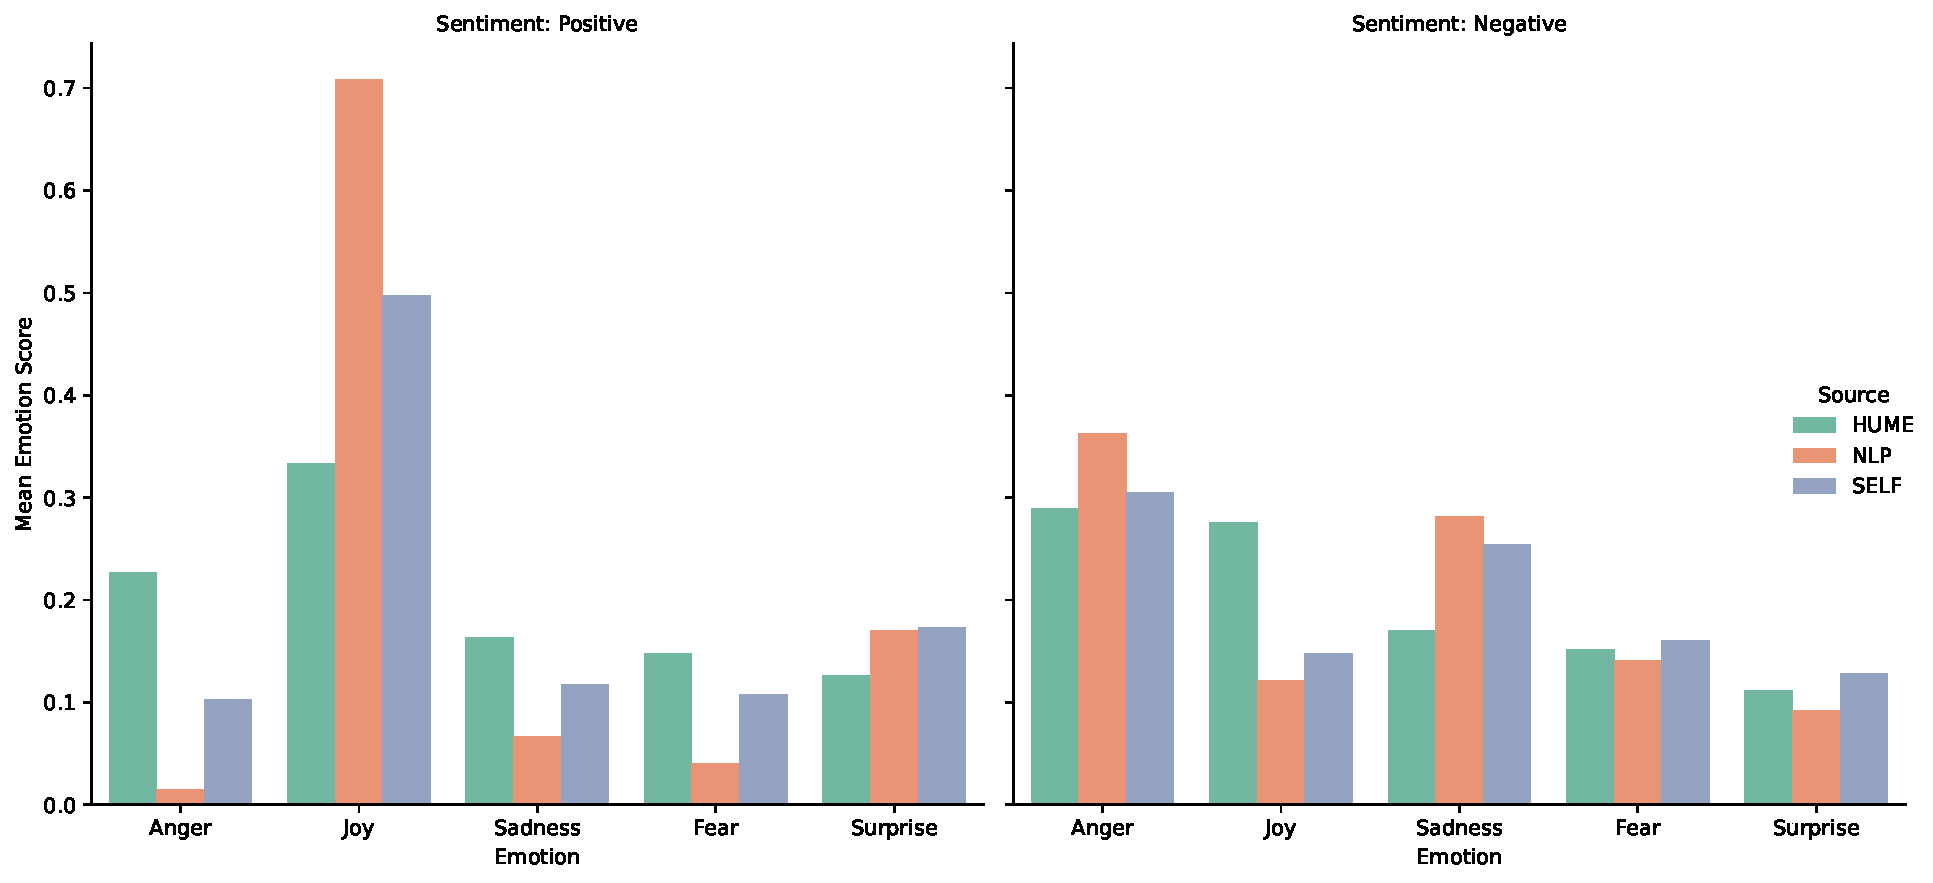
\includegraphics[width=0.7\textwidth]{png/results/rq3/rq3_sentiment_grouped_bar.pdf}
    \caption{Emotion scores for all sources grouped by sentiment.}
    \label{fig:sentiment-bar-rq3}
\end{figure}

\textbf{Positive Interviews}
\begin{itemize}
    \item Joy was highly self-reported consistently, which aligns closely with NLP Cloud's text-based ratings, but considerably higher than Hume AI's vocal analysis. 
    This alignment suggest that participants expressed positive emotions verbally, which was captured by NLP Cloud effectively. The lower Hume ratings for Joy indicate a divergence since vocal expressions of Joy in 
    the reflective, interview setting may be less pronounced and therefore harder for the speech-based model to detect. 
    \item The negative emotions (Anger, Sadness, Fear) were assessed at lower levels by participants, as expected for positive oriented interviews. Self-assessments generally matched Hume's higher detection of subtle negative emotion expressions better than NLP's minor ratings. 
    This aligns with the idea that participants may express suble negative tones unintentionally in their voice, even if the participants perceived their emotions as predonimantly positive. 
    \item Surprise showed moderate self-report levels, more close agreed to NLP and slighly less alignment with Hume, reflecting inconsistency in vocal vs. textual emotion cues.  
\end{itemize}
In positive interviews, NLP Cloud consistently rated Joy higher, in agreement with previous results. The difference from self-reported joy is similar, although NLP tends to rate it moderately higher. 
This reflect the strength of text-based detection for explicit positive sentiment when analyzed as a transcription. 

\medskip
\textbf{Negative Interviews}
\begin{itemize}
    \item Anger and Sadness were reported at higher levels by participants, which reflects the intention of the interview of recalling negative emotions. Both AI models were aligned with self-reports for Anger, even if NLP rated it somewhat higher, 
    probably due to explicit negative language in transcriptions. Sadness showed stronger alignment with NLP than Hume, indicating explicit expressed sadness-related emotions verbally. 
    \item Joy was reported low by participants, but frequently assigned higher by Hume than the other sources. Suggesting that vocal features were interpreted as positive by Hume might not align with subjective emotional experiences, 
    showing a clear divergence between vocal emotion cures and participants own perception. 
    \item Fear and Surprise showed low levels consistently across self-reports and both AI-models, indicating that these emotions were less expressed or experiences, resulting in minimal discrepancies. 
\end{itemize}

These results emphasize that emotional expression is complex in conversational settings, showing that textual anlyses track explicit articulated emotions, 
while speech-based analyses reveal less intentionally expressed emotional nuances, sometimes in disagreement with participants subjective assessments. 

The sentiment-based comparison clearly presents that emotional expression and self-awareness have a signficant variance between modalities. Explicit emotions articulated in words are closely aligned between self-assessed rating and text-based analysis. 
While implicit or suble emotions expressed through vocal tone have a notable divergence. This highlights that AI modalities complement rather than duplicate emotional understanding. 
Speech-based models provide insights into emotional subtleties that might be unconscious to the participant, while text-based analyses capture verbalized emotions closely to subjective experiences. 


\subsection{Conclusion of RQ3 Data Analysis}
The results show that both systems have partial alignment with self-reported emotions, however, the correlation varies depending on emotion and modality. 
Text-based (NLP Cloud) presented a strong alignment with participants own perception for clear verbally expressed emotions like Joy And Anger. Subtler vocal cues were interpreted by the speech-based 
model (Hume AI), which may not always reflect self-perceived emotions. Emotions like Fear and Surprise had most visiable differences for both AI models. 
Overall, the results implies that speech- and text-based emotion recognition comprehend different layers of expressed emotions, suggesting that complementary use of modalities can offer a more nuanced understanding.  